\documentclass[a4paper]{article}

\usepackage[english]{babel}
\usepackage{amsmath}
\usepackage{color}
\usepackage{amssymb}
\usepackage{dsfont}
\usepackage{multicol}
%\usepackage[lofdepth,lotdepth]{subfig}  This gives errors when used together with "subcaption", which is needed to create subfigures.
\usepackage{graphicx}
\usepackage{listings}
\usepackage[hyphens]{url}
\usepackage{pgf, tikz}
\usetikzlibrary{arrows, automata}
\usepackage{titling}
\usepackage{varwidth}
\usepackage{hyperref}
\usepackage{color} %red, green, blue, yellow, cyan, magenta, black, white
\definecolor{mygreen}{RGB}{28,172,0} % color values Red, Green, Blue
\definecolor{mylilas}{RGB}{170,55,241}
\setlength\parindent{0pt}
\usepackage{float}
\usepackage{subcaption}
\usepackage{polynom}
\usepackage{physics}
\newcommand\tab[1][1cm]{\hspace*{#1}}


\newcommand\independent{\protect\mathpalette{\protect\independenT}{\perp}}
\def\independenT#1#2{\mathrel{\rlap{$#1#2$}\mkern2mu{#1#2}}}

\usepackage{geometry}
 \geometry{
 a4paper,
 total={165mm,257mm},
 left=20mm,
 top=20mm,
 }

\definecolor{codegreen}{rgb}{0,0.6,0}
\definecolor{codegray}{rgb}{0.5,0.5,0.5}
\definecolor{codepurple}{rgb}{0.58,0,0.82}
\definecolor{backcolour}{rgb}{0.95,0.95,0.92}

\lstdefinestyle{mystyle}{
    backgroundcolor=\color{backcolour},   
    commentstyle=\color{codegreen},
    keywordstyle=\color{magenta},
    numberstyle=\tiny\color{codegray},
    stringstyle=\color{codepurple},
    basicstyle=\footnotesize,
    breakatwhitespace=false,         
    breaklines=true,                 
    captionpos=b,                    
    keepspaces=true,                 
    numbers=left,                    
    numbersep=5pt,                  
    showspaces=false,                
    showstringspaces=false,
    showtabs=false,                  
    tabsize=2
}
 
\lstset{style=mystyle}


\DeclareMathOperator*{\argmax}{arg\,max}
\DeclareMathOperator*{\argmin}{arg\,min}

\title{Statistical Machine Learning 2018\\Assignment 3\\Deadline: 25th of November 2018}
\author{
  Christoph Schmidl\\ s4226887\\      \texttt{c.schmidl@student.ru.nl}
  \and
  Mark Beijer\\ s4354834\\     \texttt{mbeijer@science.ru.nl}
}
\date{\today}

\begin{document}
\maketitle


\section*{Exercise 1 - The faulty lighthouse (weight 5)}

A lighthouse is somewhere off a piece of straight coastline at a position $\alpha$ along the shore and a distance $\beta$ out to sea. Due to a technical fault, as it rotates the light source only occasionally and briefly flickers on and off. As a result it emits short, highly focused beams of light at random intervals. These pulses are intercepted on the coast by photo-detectors that record only the fact that a flash has occurred, but not the angle from which it came. So far, $N$ flashes have been recorded at positions $\mathcal{D} = {x1, . . . , xN }$. Where is the lighthouse?

\begin{figure}[H]
\center
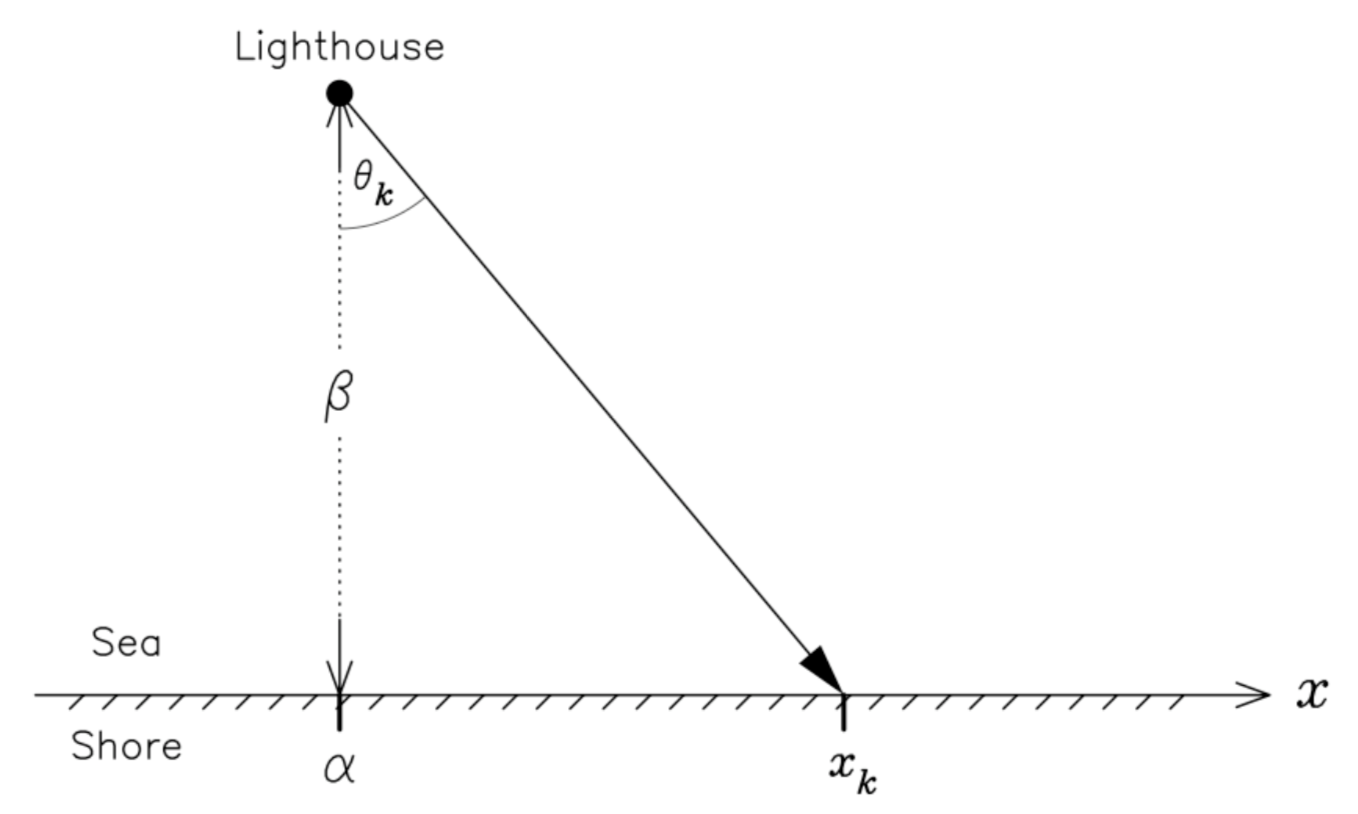
\includegraphics[width=0.75\textwidth]{Images/lighthouse_fig.png}
\caption{Geometry of the lighthouse problem.}
\label{Fig:lighthouse}
\end{figure}




\textbf{Part 1 - Constructing the model}\\

\subsection*{1.1.1}

Let $\theta_k$ be the (unknown) angle for the k-th recorded flash, see fig.1. Argue why

\begin{eqnarray}
p(\theta_k | \alpha, \beta) = \frac{1}{\pi}
\end{eqnarray}

would be a reasonable distribution over $\theta_k$ between $\pm \frac{\pi}{2}$ (zero otherwise).\\


\textbf{Answer:}\\

The description states that photo-detectors are only located on the coast side but not on the shore side. Normally a lighthouse emits light in a rotating fashion of $360^{\circ}$ but based on the before mentioned fact we can assume that photo-detectors can only detect light beams in an angle of $180^{\circ}$ around the light house on the coast side, whereas the remaining $180^{\circ}$ on the shore side are not detected by any photo-detectors. If we transform the degrees into radians then we have $360^{\circ} = 2 \pi $ radians and $180^{\circ} =  \pi $ radians. Based on the fact that we are only interested in the specific angle $\theta_k$ and not the whole region of $180^{\circ}$ or $\pi$ radians, $\frac{1}{\pi}$ seems like a reasonable distribution in this case.\\

We can also show that $p(\theta_k | \alpha, \beta) = \frac{1}{\pi}$ is a reasonable distribution over $\theta_k$ between $\pm \frac{\pi}{2}$ by demsonstrating that it integrates to 1:

\begin{align*}
\int_{-\frac{\pi}{2}}^{\frac{\pi}{2}} \frac{1}{\pi}  \: dx &= \bigg[ \frac{x}{\pi} \bigg]_{-\frac{\pi}{2}}^{\frac{\pi}{2}}\\
&= \big[ \frac{\frac{\pi}{2}}{\pi} \big] - \big[- \frac{\frac{\pi}{2}}{\pi} \big]\\
&= \frac{\frac{\pi}{2} + \frac{\pi}{2}}{\pi}\\
&= \frac{\pi}{\pi}\\
&= 1
\end{align*}

\subsection*{1.1.2}

We only have the position $x_k$ of the detector that recorded flash $k$, but we can relate this to the unknown $\theta_k$ via elementary geometry as

\begin{eqnarray}
\beta \tan(\theta_k) = x_k - \alpha	
\end{eqnarray}

Show that the expected distribution over $x$ given $\alpha$ and $\beta$ can be written as

\begin{eqnarray}
p(x_k | \alpha, \beta) = \frac{\beta}{\pi [\beta^2 + (x_k - \alpha)^2 ]}
\end{eqnarray}

by using (2) to substitute variable $x_k$ for $\theta_k$ in the distribution (1). Plot the distribution for $\beta = 1$ and a particular value of $\alpha$.\\
Hint: use the Jacobian $|\frac{d \theta}{d x }|$ (Bishop, p.18) and the fact that $(tan^{-1}x)' = \frac{1}{1 + x^2}$.\\



\textbf{Answer:}\\

Isolating variable $\theta_k$ using arctan:

\begin{align*}
\beta \tan(\theta_k) &= x_k - \alpha\\
\tan(\theta_k) &= \frac{x_k - \alpha}{\beta}\\
\theta_k &= \tan^{-1}(\frac{x_k - \alpha}{\beta})
\end{align*}

Computing the jacobian and using the little hint that $(tan^{-1}x)' = \frac{1}{1 + x^2}$:

\begin{align*}
|\frac{d \theta}{d x }| &= \frac{1}{1 + (\frac{x_k - \alpha}{\beta})^2} \times \frac{\beta}{\beta^2}\\
&= \frac{\beta}{\beta^2 + \beta^2(\frac{x_k - \alpha}{\beta})^2}\\
&= \frac{\beta}{ \beta^2 + (x_k - \alpha)^2}
\end{align*}

Showing that the expected distribution over $x$ given $\alpha$ and $\beta$ can be written as

\begin{align*}
p(x_k | \alpha, \beta) = \frac{\beta}{\pi [\beta^2 + (x_k - \alpha)^2 ]}
\end{align*}

by:

\begin{align*}
p(x_k | \alpha, \beta) &= p(\theta_k) \times \big| \frac{d \theta}{d x} \big|\\
&= \frac{1}{\pi} \times  \frac{\beta}{ \beta^2 + (x_k - \alpha)^2}\\
&= \frac{\beta}{\pi [\beta^2 + (x_k - \alpha)^2 ]}
\end{align*}

Plotting the distribution as shown in figure \ref{fig:112} using the following code:

\begin{lstlisting}[language=Python]
import numpy as np
import matplotlib.pyplot as plt 
%matplotlib inline

def get_probability_distribution(x, alpha, beta):
    return beta/(np.pi*(beta**2+(x-alpha)**2))
    
x = np.linspace(-10, 10, num=1000) 
probs = get_probability_distribution(x, 3, 1) 
plt.xlabel(r'$x_k$')
plt.ylabel(r'$p(x_k|\alpha, \beta)$')
plt.plot(x, probs)
plt.savefig('1_1_2.png')
plt.show()    
\end{lstlisting}

\begin{figure}[H]
\center
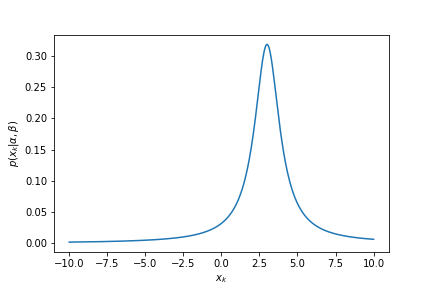
\includegraphics[width=0.6\textwidth]{Images/1_1_2.png}
\caption{Plotting $p(x_k | \alpha, \beta)$ with $\alpha = 3$ and $\beta = 1$}
\label{fig:112}
\end{figure}

\subsection*{1.1.3}

Inferring the position of the lighthouse corresponds to estimating $\alpha$ and $\beta$ from the data $\mathcal{D}$. This is still quite difficult, but if we assume that $\beta$ is known, then from Bayes’ theorem we know that $p(\alpha|\mathcal{D}, \beta) \propto p(\mathcal{D}|\alpha, \beta) p(\alpha|\beta)$. We have no a priori knowledge about the position $\alpha$ along the coast other than that it should not depend on the distance out at sea.\\

Show that with these assumptions the log of the posterior density can be written as

\begin{eqnarray}
L = \ln (p(\alpha | \mathcal{D, \beta})) = \texttt{constant} - \sum_{k = 1}^N \ln [\beta^2 + (x_k - \alpha)^2] 
\end{eqnarray}

and give an expression for the value $\hat{\alpha}$ that maximizes this posterior density.\\

\textbf{Answer:}\\

\begin{align*}
L &= \ln(p(\alpha|\mathcal{D}, \beta))\\
&= \ln(\prod_{k=1}^N \frac{\beta}{\pi [\beta^2 + (x_k - \alpha)^2]})\\
&= \sum_{k=1}^N \ln (\frac{\beta}{\pi} \times \frac{1}{\beta^2 + (x_k - \alpha)^2})\\
&= N \ln \frac{\beta}{\pi} - \sum_{k=1}^N \ln [\beta^2 + (x_k - \alpha)^2]\\
&= constant - \sum_{k = 1}^N \ln [\beta^2 + (x_k - \alpha)^2]
\end{align*}

Expression for the value $\hat{\alpha}$ that maximizes this posterior density:

\begin{align*}
\hat{\alpha} = \argmax_\alpha \sum_{k = 1}^N \ln [\beta^2 + (x_k - \alpha)^2]
\end{align*}

\subsection*{1.1.4}

Suppose we have a data set (in km) of $\mathcal{D} = \{ 3.6, 7.7, -2.6, 4.9, -2.3, 0.2, -7.3, 4.4, 7.3, -5.7\}$. We also assume that the distance $\beta$ from the shore is known to be 2 km. As it is difficult to find a simple expression for the value of $\hat{\alpha}$ that maximizes (4), we try an alternative approach instead.\\

Plot $p(\alpha|\mathcal{D}, \beta = 2)$ as a function of $\alpha$ over the interval $[-10, 10]$. What is your most likely estimate for $\hat{\alpha}$ based on this graph? Compare with the mean estimate of the dataset. Can you explain the difference?\\


\textbf{Answer:}\\




\textbf{Part 2 - Generate the lighthouse data}\\


We will try to solve the original problem by letting matlab/Python find the lighthouse for us. For that we first need a data set.

\subsection*{1.2.1}

Sample a random position $(\alpha_t, \beta_t)$ from a uniform distribution over an interval of 10 km along the coast and between 2 and 4 km out to sea.\\

\textbf{Answer:}\\


\subsection*{1.2.2}

From this position generate a data set $\mathcal{D} = \{ x_1,..., x_N \}$ of 500 flashes in random directions that have been registered by a detector at point $x_i$ along the coast. Assume that the flashes are i.i.d. according to (1).\\

\textbf{Answer:}\\


\subsection*{1.2.3}

Make a plot of the mean of the data set as a function of the number of points. Compare with the true position of the lighthouse $\alpha_t$. How many points do you expect to need to obtain a reasonable estimate of $\alpha_t$ from the mean? Explain.\\

\textbf{Answer:}\\



\textbf{Part 3 - Find the lighthouse}\\

From the analysis in the first part we know that trying to find a maximum likelihood estimate in the usual way is possible (compute gradient, set equal to zero and solve), but that this does not result in a ‘nice’ closed-form expression for the solution, even when one of the parameters is assumed to be known. As we want to find estimates of both $\alpha$ and $\beta$ from the data, we will try a different approach instead.

\subsection*{1.3.1}

Use (3) to get an expression for the loglikelihood of the data $\mathcal{D}$ as a function of $\alpha$ and $\beta$.\\

\textbf{Answer:}\\


\subsection*{1.3.2}

We can see how this likelihood (as a function of $\alpha$ and $\beta$) changes, as data points come in.\\

Process your data set $\mathcal{D}$ one by one and make a plot of the (log)likelihood after one, two, three, and 20 points have arrived, respectively. Explain what happens.\\

Hint: Create a function that calculates the (log)likelihood at a specific point $(\alpha, \beta)$ after the first $k$ data points $\{x_1, . . . , x_k \}$ have come in. Use this with the matlab \texttt{ meshgrid} and \texttt{surf}  functions to make plots over the interval $[-10 \leq \alpha \leq +10] \times [0 \leq \beta \leq 5]$. Decide if/when it makes more sense to use the likelihood directly or the log of the likelihood.\\

\textbf{Answer:}\\



\subsection*{1.3.3}

We can make a reasonable (visual) estimate of the most probable position of the lighthouse from the graph, after a few data points have been observed. However, as we are working with a computer, we will let matlab do the dirty work for us.\\

Create a function that uses matlab function \texttt{fminsearch} to compute the values of $\alpha$ and $\beta$ that maximize the likelihood for a data set of $k$ points, and plot these as a function of the number of points. Use $[0, 1]$ as the initial starting value for \texttt{ fminsearch} (see examples in matlab-help). Compare your final estimate with the true values $(\alpha_t,\beta_t)$.\\

\textbf{Answer:}\\



\section*{Exercise 2 - Bayesian linear regression (weight 2)}

This exercise builds on exercise 2, week 7, “Fitting a straight line to data”. For a detailed de- scription (and explanation) see Exercises and Answers, Week 7 in Brightspace. The final part of that exercise computed the predictive distribution after a single data point was observed. Here we consider a new data set, consisting of no less than two points: ${x_1,t_1} = (0.4,0.1)$ and ${x_2, t_2} = (0.6, -0.4)$.


\subsection*{2.1}

Assume $\alpha = 1$ and $\beta = 15$. Compute the predictive distribution $p(t|x, \textbf{t}, \textbf{x}, \alpha, \beta)$ after these two points are observed.\\

\textbf{Answer:}\\


\subsection*{2.2}


Plot the mean of the predictive Gaussian distribution and one standard deviation on both sides as a function of $x$ over the interval $[0,1]$. Plot the data in the same figure. See \texttt{a009plotideas.m} in Brightspace for some plotting hints. Compare your plot with Figure 3.8b (Bishop, p.157) and explain the difference.\\

\textbf{Answer:}\\



\subsection*{2.3}

Sample five functions $y(x,\textbf{w})$ from the posterior distribution over $\textbf{w}$ for this data set and plot them in the same graph (i.e. with the predictive distribution). You may use the Matlab function \texttt{mvnrnd}. See again \texttt{a009plotideas.m} for some plotting hints.\\

\textbf{Answer:}\\



\section*{Exercise 3 - Gradient descent revisited (weight 3)}

In this exercise, we will have a closer look at the gradient descent algorithm for function minimization. When the function to be minimized is $E(x)$, the gradient descent iteration is


\begin{eqnarray}
\textbf{x}_{n + 1} = \textbf{x}_n - \eta \nabla E(\textbf{x}_n)
\end{eqnarray}

where $\eta > 0$ is the so-called learning-rate.

\subsection*{3.1}

Consider the function $f(x) = \frac{\lambda}{2}(x - a)^2$ with parameters $\lambda > 0$, and $a$ arbitrary.


\subsection*{3.1a}

Write down the gradient descent iteration rule. Verify that the minimum of $f$ is a fixed point\footnote{A fixed point $x^*$ of an iteration $x_{n+1} = F(x_n)$ satisfies $x^* = F(x^*)$.} of the gradient descent iteration rule.\\

\textbf{Answer:}\\

The gradient of f is:

\begin{equation}
\nabla f(x) = \lambda (x-a)
\end{equation}

And therefore the gradient descent iteration rule is:

\begin{equation}
x_{n+1} = x_n - \eta \lambda (x_n-a)
\end{equation}

The minimum of f can be found by setting it's gradient to 0:

\begin{eqnarray}
\lambda(x-a) &=& 0\\
x-a &=& 0 \\
x &=& a
\end{eqnarray}

To show it's a minimum we can take the second derivitive at point a:

\begin{equation}
f''(x) = \lambda \rightarrow f''(a) = \lambda
\end{equation}

Since $\lambda$ is strictly greater then 0, the second derivative at a is strictly greater then 0 and therefor a is the minimum.

a is a fixed point since:

\begin{eqnarray}
x_{n+1} &=& a - \eta \nabla f(a)\\
&=& a - \eta \lambda (a-a) = a
\end{eqnarray}

\subsection*{3.1b}

Find $\eta$ for which convergence is the fastest (actually in one step).\\

\textbf{Answer:}\\

Since it is given that the fastest is in one step, we can write :

\begin{eqnarray}
a &=& x - \eta \lambda f(x)\\
&=& x - \eta \lambda (x-a)\\
\eta \lambda (x-a) &=& x - a\\
\eta \lambda &=& 1\\
\eta &=& \frac{1}{\lambda}
\end{eqnarray}

You can also see this by looking at the iteration rule. Since when $\eta = \lambda^{-1}$, in the next iteration $x_n$ will cancel and you're left with (-(-a))=a, thus arriving at the minimum in one step, independent of x. 

\subsection*{3.1c}

We will investigate the convergence properties for different values of $\eta$. For this we look at the ratio of the distance to the fixed point after the step and the distance before the step:
 
\begin{eqnarray}
r_n = \frac{|x_{n+1} - x^*|}{|x_n - x^*|}
\end{eqnarray}

\subsubsection*{3.1c.i}

What does it mean if all $r_n < c < 1$ (i.e. all ratio’s are smaller than a certain number below 1). Give for this case the (optimal) upper bound of the distance $|x_n - x^*|$ in terms of $|x_0 - x^*|$ , $c$ and $n$.\\

\textbf{Answer:}\\

If for all $r_n < c < 1$ then it means that always, independent of the iteration step, beginning starting point $x_0$, the ratios of the next iteration and the current are always lower then some number strictly smaller then 1. This means that the distance $r_n$ to the fixed point always decreases with a rate bounded by c. It also means that every new step brings you closer to a, it's not like there is some other fixed point you might end up at.
\newpage 
At every step the distance is multiplied by at least c, since the difference between the distance of the current and next step is c or lower. So the upper bound on the distance would be:

\begin{equation}
\abs{x_n-x^*} = c^n \abs{x_0 - x^{*}}
\end{equation}

Note that $c^n < 1$ since $ 0 < c < 1$.


\subsubsection*{3.1c.ii}

What is the consequence if all $r_ > c > 1$? Give for this case the optimal lower bound of the distance $|x_n - x^*|$ in terms of $|x_0 - x^*|$, $c$ and $n$.\\

\textbf{Answer:}\\


Then with every step you get further and further away from the optimal point $x^*$. Therefore you'll diverge from the point $x^*$. The constant c is larger than 1, so it is bounded by 1. While c can't be 1, it is the lower bound. Taking this we get that the best case scenario the distance won't change, so we get:

\begin{equation}
\abs{x_n-x^*} = \abs{x_0-x^*} + \epsilon
\end{equation}

With $0 < \epsilon$.

\subsection*{3.1d}

Show that in our case, $r_n = |1 - \eta \lambda| \equiv r$, independent of $n$ (we refer to $r$ as the convergence rate). For which $\eta$ is the algorithm convergent?\\

\textbf{Answer:}\\

\begin{eqnarray}
r_n &=& \frac{\abs{x_{n+1} - x^*}}{\abs{x_n - x^*}}\\
&=& \frac{\abs{ x_n - \eta \lambda (x_n - a) - a}}{\abs{x_n - a}}\\
&=& \frac{\abs{(1-\eta \lambda) (x_n - a)}}{\abs{x_n - a}}\\
&=& \abs{1-\eta \lambda}
\end{eqnarray}


This converges for when $r_n$ is strictly smaller then 1, so when $0 < \eta \lambda < 2$. So:

\begin{equation}
0 < \eta < \frac{2}{\lambda }
\end{equation}




\subsection*{3.2}

Consider the function $g(x, y) = \frac{\lambda_1}{2}(x - a_1)^2 + \frac{\lambda_2}{2} (y - a_2)^2$ with parameters $0 < \lambda_1 \leq \lambda_2$, and $a_i$ arbitrary.

\subsection*{3.2a}

Write down the gradient descent iteration rule. Verify that the minimum of $f$ is a fixed point.\\

\textbf{Answer:}\\

The gradient of the function g is:

\begin{eqnarray}
\pdv{g}{x} &=& \lambda_1(x-a_1)\\
\pdv{g}{y} &=& \lambda_2(y-a_2)\\
\nabla g &=& \begin{bmatrix}
\pdv{g}{x}\\
\pdv{g}{y}
\end{bmatrix} = \begin{bmatrix}
\lambda_1 (x-a_1)\\
\lambda_2 (y-a_2)
\end{bmatrix}\\
\begin{bmatrix}
x_{n+1}\\
y_{n+1}
\end{bmatrix} &=& \begin{bmatrix}
x_n\\
y_n
\end{bmatrix} -  \eta \nabla g(x_n)\\
&=& \begin{bmatrix}
x_n\\
y_n
\end{bmatrix} - \eta \begin{bmatrix}
\lambda_1 (x_n-a_1)\\
\lambda_2 (y_n-a_2)
\end{bmatrix}
\end{eqnarray}

The minimum of g is: (I think the f was a typing error)

\begin{eqnarray}
\nabla g  &=& \begin{bmatrix}
0\\
0
\end{bmatrix}\\
&=& \begin{bmatrix}
\lambda_1 (x-a_1)\\
\lambda_2 (y-a_2)
\end{bmatrix}\\
\lambda_1 (x-a_1) &=& 0 \rightarrow x = a_1\\
\lambda_2 (y-a_2) &=& 0 \rightarrow y = a_2\\
\end{eqnarray}

Now to show it is a fixed point:

\begin{eqnarray}
\begin{bmatrix}
x_{n+1}\\
y_{n+1}
\end{bmatrix} &=& \begin{bmatrix}
a_1\\
a_2
\end{bmatrix} - \eta \begin{bmatrix}
\lambda_1 (a_1-a_1)\\
\lambda_2 (a_2-a_2)
\end{bmatrix}\\
&=& \begin{bmatrix}
a_1\\
a_2
\end{bmatrix}
\end{eqnarray}


\subsection*{3.2b}

Show that $\eta = \frac{2}{\lambda_2 + \lambda_1}$ minimizes the larger ratio between $r_{n,x} = \frac{|x_{n+1} - x^*|}{|x_n - x^*|}$ and 	$r_{n,y} = \frac{|y_{n+1} - y^*|}{|y_n - y^*|}$, i.e., $\argmin_\eta \{ max\{r_{n,x},r_{n,y} \} \} = \frac{2}{\lambda_2 + \lambda_1}$. What happens if $\eta$ is smaller than this optimal value? What happens if it is larger?\\

\textbf{Answer:}\\


For the first ratio:

\begin{eqnarray}
r_{n,x} &=& \frac{\abs{x_{n+1}- x^*}}{\abs{x_n - x^*}}\\
&=& \frac{\abs{x_n - \eta\lambda_1 (x_n-a_1) - a_1}}{\abs{x_n - a_1}}\\
&=& \frac{\abs{ (1- \eta \lambda_1) (x_n - a_1)}}{\abs{x_n - a_1}}\\
&=& \abs{1-\eta \lambda_1}
\end{eqnarray}

For the second ratio:

\begin{eqnarray}
r_{n,y} &=& \frac{\abs{y_{n+1}- y^*}}{\abs{y_n - y^*}}\\
&=& \frac{\abs{y_n - \eta\lambda_2 (y_n-a_2) - a_2}}{\abs{y_n - a_2}}\\
&=& \frac{\abs{ (1- \eta \lambda_2) (y_n - a_2)}}{\abs{y_n - a_2}}\\
&=& \abs{1-\eta \lambda_2}
\end{eqnarray}

When they are at the minimum, the values are equal. For if one is not equal but higher you can always go in one direction to lower the first until it lowers so much it equals the second. This is easier to understand by looking at an example plot, here $\lambda_1 = 1$ and $\lambda_2 = 2$.

\begin{figure}[H]
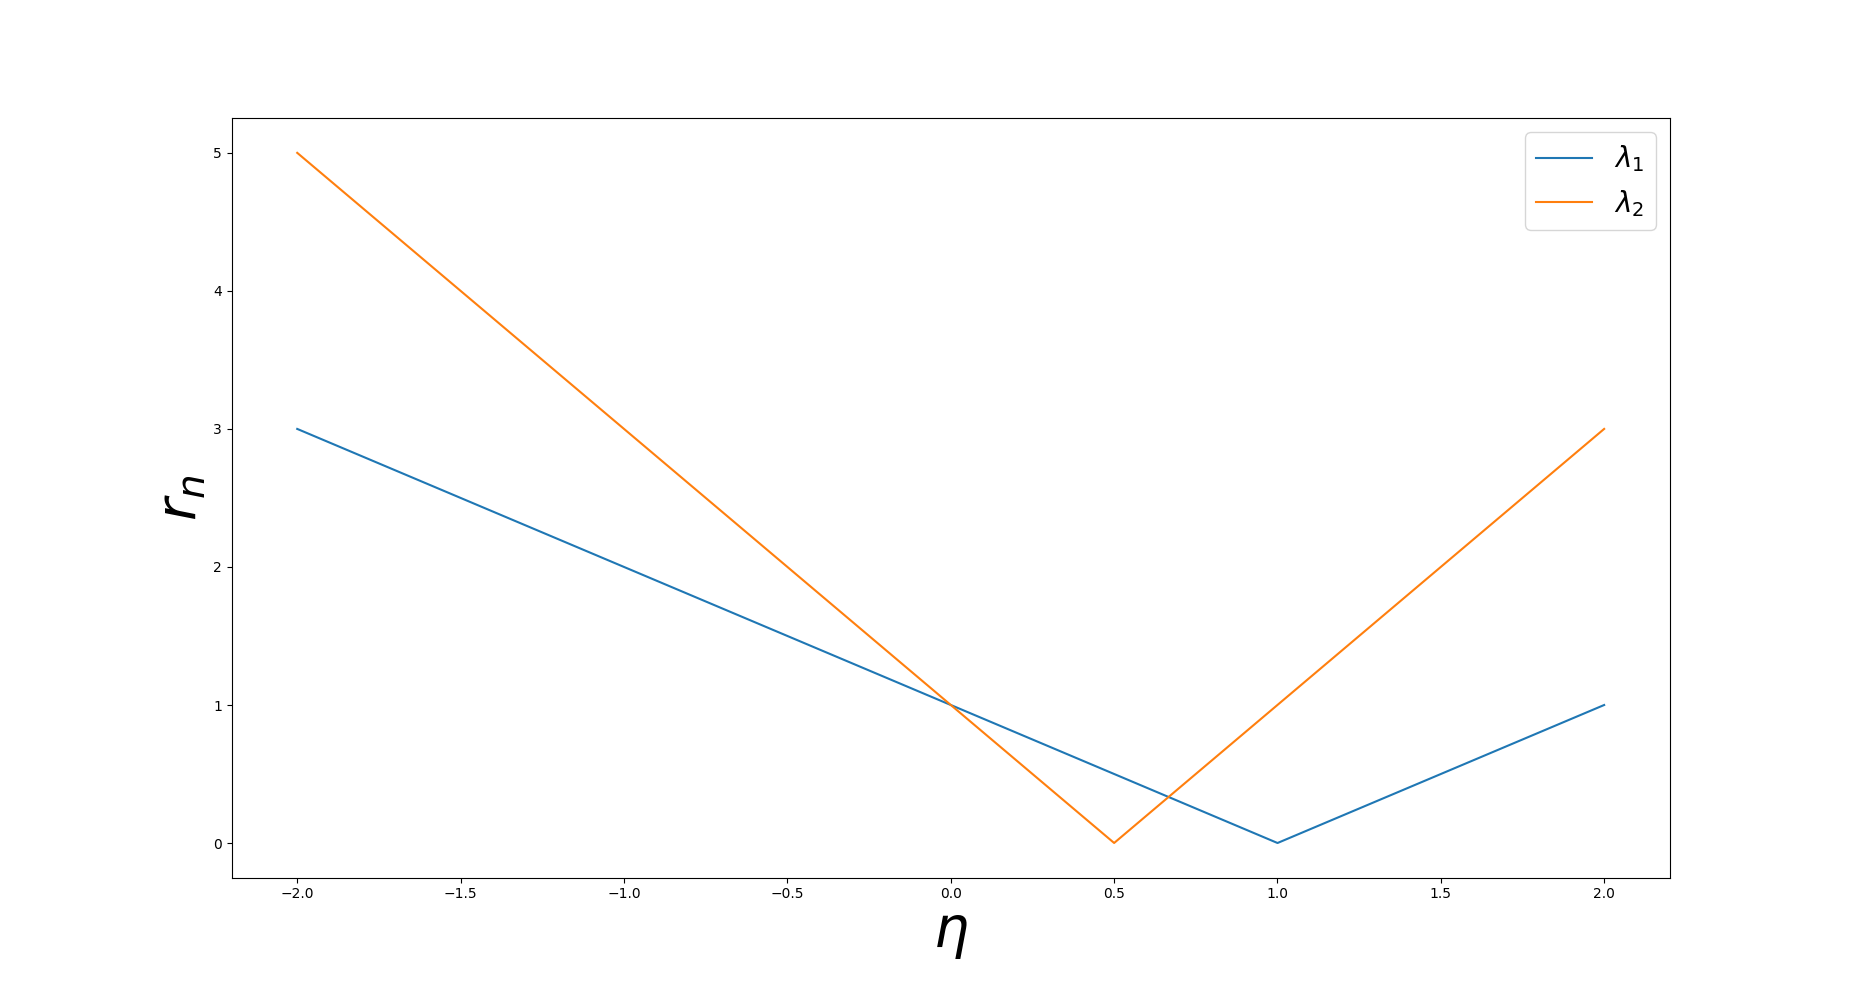
\includegraphics[width=\textwidth]{Images/32b.png}
\caption{Two ratios for $\lambda_1 = 1$ and $\lambda_2$ = 2. Notice that the optimal value is found at the second intersection, where $\eta \neq 0$, for the highest value of both of the functions is the lowest, moving left or right of that point either one is higher then at the intersection.}
\label{Converg}
\end{figure}

\begin{eqnarray}
\abs{1-\eta \lambda_1} &=& \abs{1-\eta \lambda_2}\\
(1-\eta \lambda_1)^2 &=& (1- \eta \lambda_2)^2\\
1 - \eta \lambda_1 &=& \pm (1-\eta \lambda_2)\\
1 - \eta \lambda_1 &=& 1 - \eta \lambda_2\\
\eta \lambda_2 - \eta \lambda_1 &=& 0 \\
\eta &=& 0 \tab \text{Not the lowest solution, let's try the -}\\
1 - \eta \lambda_1 &=& \eta \lambda_2 - 1\\
2 &=& \eta (\lambda_1 + \lambda_2)\\
\eta &=& \frac{2}{\lambda_1 + \lambda_2}
\end{eqnarray}

We can say without loss of generality that $\lambda_1 < \lambda_2$. If that's not the case we can either swap lables. If they are the same then the ideal rate is optimal in both dimensions, and using an $\eta$ different then the optimal will decrease the converging rate for both directions x and y.

As we can see in figure $\ref{Converg}$, a value of $\eta$ which is lower then the optimal will make y converge faster, though if it's negative it would make x diverge not as fast. If $\eta$ is greater then the optimal value, x will converge faster and after some point diverge slower then y.

\newpage
\subsection*{3.2c}

What is the convergence rate for this $\eta$? What does this say about the applicability of
gradient descent to functions with steep hills and flat valleys (i.e., if $\lambda_2 \gg \lambda_1$)?\\

\textbf{Answer:}\\

The convergence rate for x and y  will be:

\begin{eqnarray}
r_{n,x} &=& \abs{1 - \frac{2\lambda_1}{\lambda_1 + \lambda_2}}\\
r_{n,y} &=& \abs{1 - \frac{2\lambda_2}{\lambda_1 + \lambda_2}}
\end{eqnarray}

In the case that $\lambda_2 \gg \lambda_1$, we can say that $\lambda_1 = \epsilon \lambda_2$. Then we can take the limit for $\epsilon \rightarrow 0$.

\begin{eqnarray}
\lim_{\epsilon \rightarrow 0} (1+\epsilon) &=& 1\\
r_{n,x} &=& \abs{1 - \frac{2\epsilon \lambda_2}{(1 + \epsilon) \lambda_2}}\\
\lim_{ \epsilon\rightarrow 0} r_{n,x} &=& \lim_{ \epsilon\rightarrow 0} \abs{1 - \frac{2\epsilon \lambda_2}{(1 + \epsilon) \lambda_2}}\\
&=& \lim_{ \epsilon\rightarrow 0} \abs{1 - \frac{2 \epsilon\lambda_2}{\lambda_2}}\\
&=& \lim_{ \epsilon\rightarrow 0} \abs{1 - 2\epsilon}\\
&=& 1
\end{eqnarray}

Now for y:

\begin{eqnarray}
r_{n,y} &=& \abs{ 1- \frac{2\lambda_2}{(1+\epsilon) \lambda_2}}\\
\lim_{ \epsilon\rightarrow 0} r_{n,y} &=& \lim_{ \epsilon\rightarrow 0} \abs{ 1- \frac{2\lambda_2}{(1+\epsilon) \lambda_2}}\\
&=& \lim_{ \epsilon\rightarrow 0} \abs{ 1- \frac{2\lambda_2}{ \lambda_2}}\\
&=& \abs{1 - 2} = 1
\end{eqnarray}

So it won't converge it either direction. 

\subsection*{3.2d}

Implement the gradient descent algorithm for g in matlab.\\

\textbf{Answer:}\\


\subsection*{3.2e}

Make some plots of the trajectories $\{(x_n,y_n)\}^N_{n=0}$ for different values of $\lambda_i$ and $\eta$ ($\eta$ optimal, larger than optimal, and smaller than optimal) to illustrate what is going on. Plot these trajectories on top of a contour plot of g. Monitor the convergence rates. Explain what happens.\\

\textbf{Answer:}\\

Let's first take an example from what we saw in 3.2c. We've chosen $\lambda_1 = 10^7$ and $\lambda_2 = 1$. We've taken $\eta$ to be the optimal value ($\frac{2}{\lambda_1 + \lambda_2}$). $x_0 = 3$ and $y_0 = 4$ for all the situations.


\begin{figure}[H]
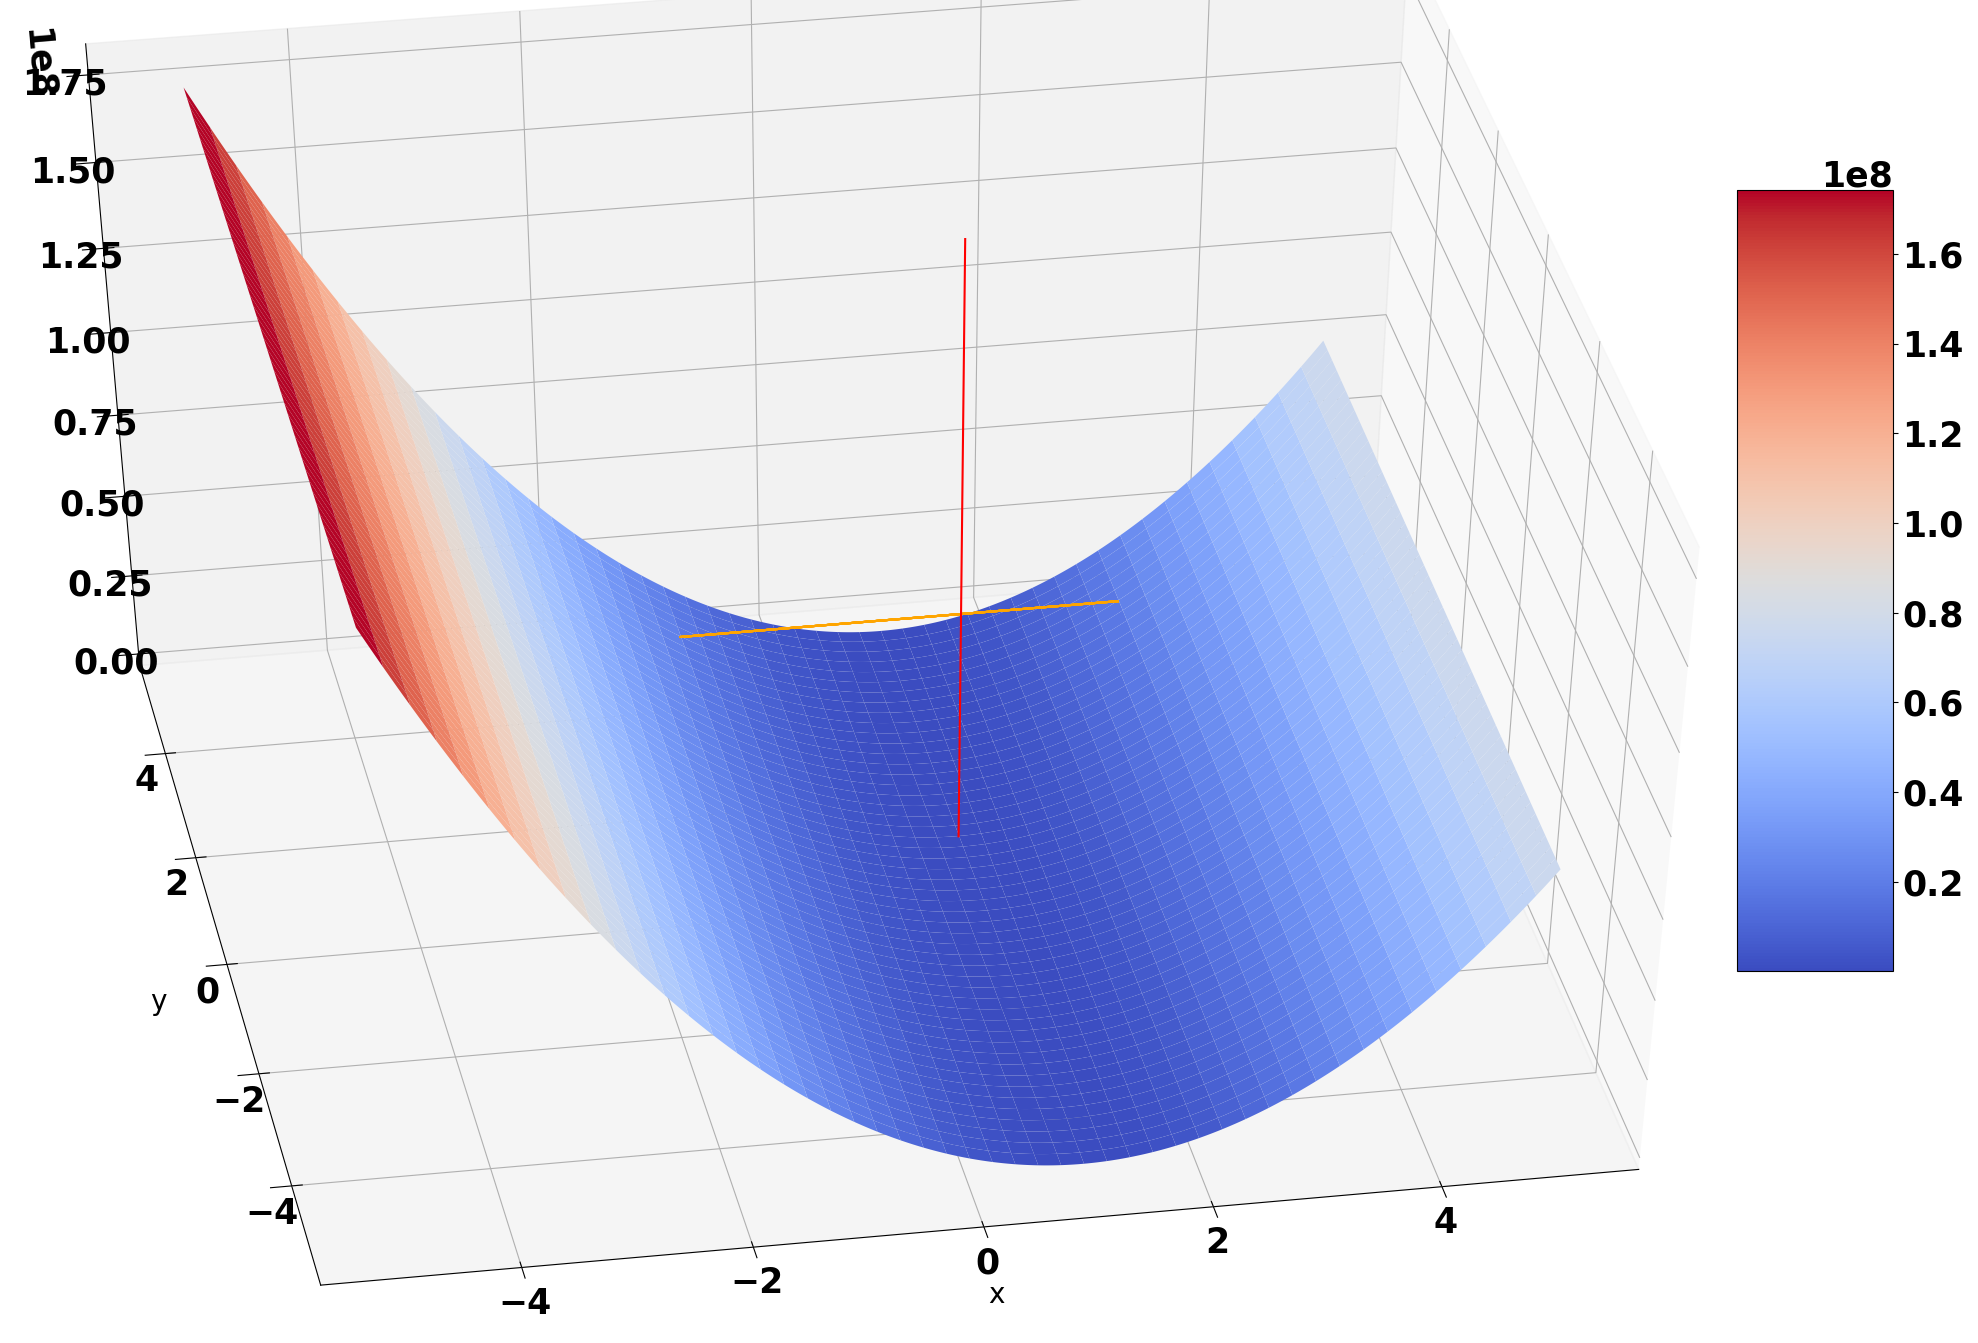
\includegraphics[width=0.7\textwidth]{Images/HighLamb.png}
\caption{Gradient descent for high $\lambda_1$. Notice how high the hill is ($10^8$). In the x direction it hops between $\approx$ 3 and $\approx$ -1. y stays at $\approx$ 4.}
\label{mountain}
\end{figure}

What happens at \ref{mountain} is that in x, $\eta \lambda$ equals 2. So it would need to go to x=1, but it overshoots by going exactly twice the required amount. So it will land on $3 - (2\cdot -2) = -1$.
From there it will overshoot going back and it will land again on $x\approx 2$. For y $\eta \lambda$ almost equals 0, so it doesn't go anywhere and stays at y=4.

I use approximate because it doesn't go exactly to -1, it first for examples goes to -0.9999996000000402. This is because it will have this behaviour in the event of $\lambda_1 \rightarrow \infty$ and we're not quite there yet for $\lambda_1 = 10^7$, but we can get arbitrary close to it if we make $\lambda_1$ larger. (This all assumes $\lambda_2$ stays the same)
\\

Another way to make it stuck forever (this time truly forever) is by chosing $\eta$ in such a way that it will always overshoot. If we take $\lambda_1 = \lambda_2 = \lambda$, then $\eta = \frac{2}{\lambda}$ will give the desired result, since then $r_n = \abs{1-\eta \lambda} = \abs{1 - 2} = 1$. An example is that for $\lambda = 1$ and $\eta = 2$. This you can see in figure \ref{NonConLamb}.

\begin{figure}[H]
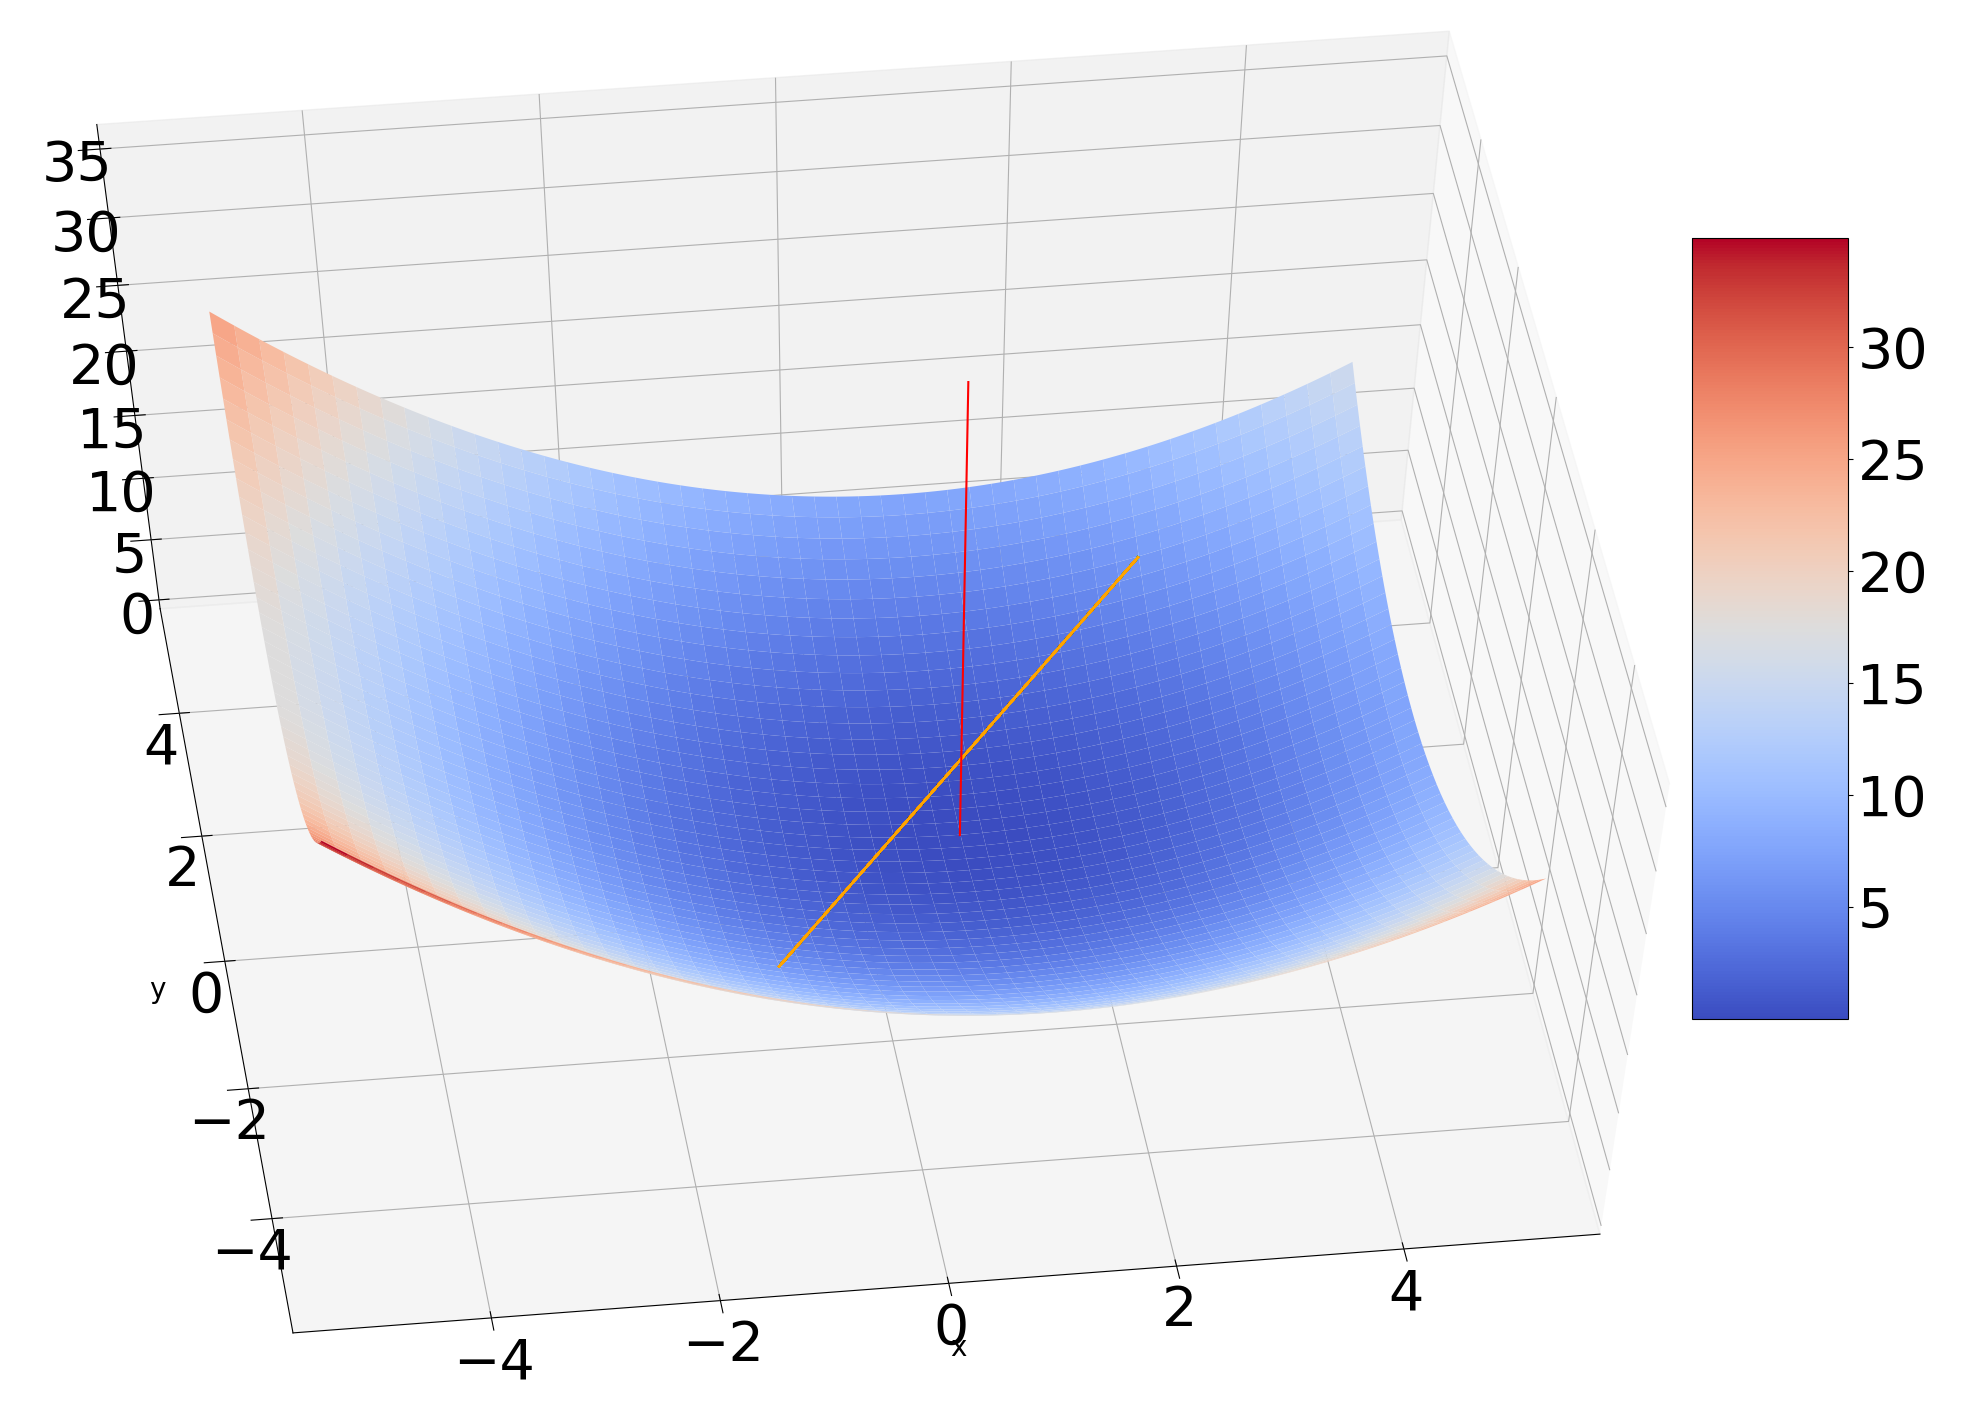
\includegraphics[width=0.7\textwidth]{Images/NonConLamb.png}
\caption{Gradient descent for $\lambda_1=\lambda_2 = 1$ and $\eta = 2$. Now the distance to the optimal point won't increase or decrease, and it jumps to and from the two only reachable points. }
\label{NonConLamb}
\end{figure}


\newpage

Now let's look at two examples of converging paths. If we set $\eta$ at the optimal value it can converge in one step if the $\lambda_1=\lambda_2$. Then for both directions the ideal $\eta$ is the same. We took $\lambda_1=\lambda_2 = 1$ and the ideal number for $\eta$. Then we get the following graph as seen in figure \ref{Ideal}.

\begin{figure}[H]
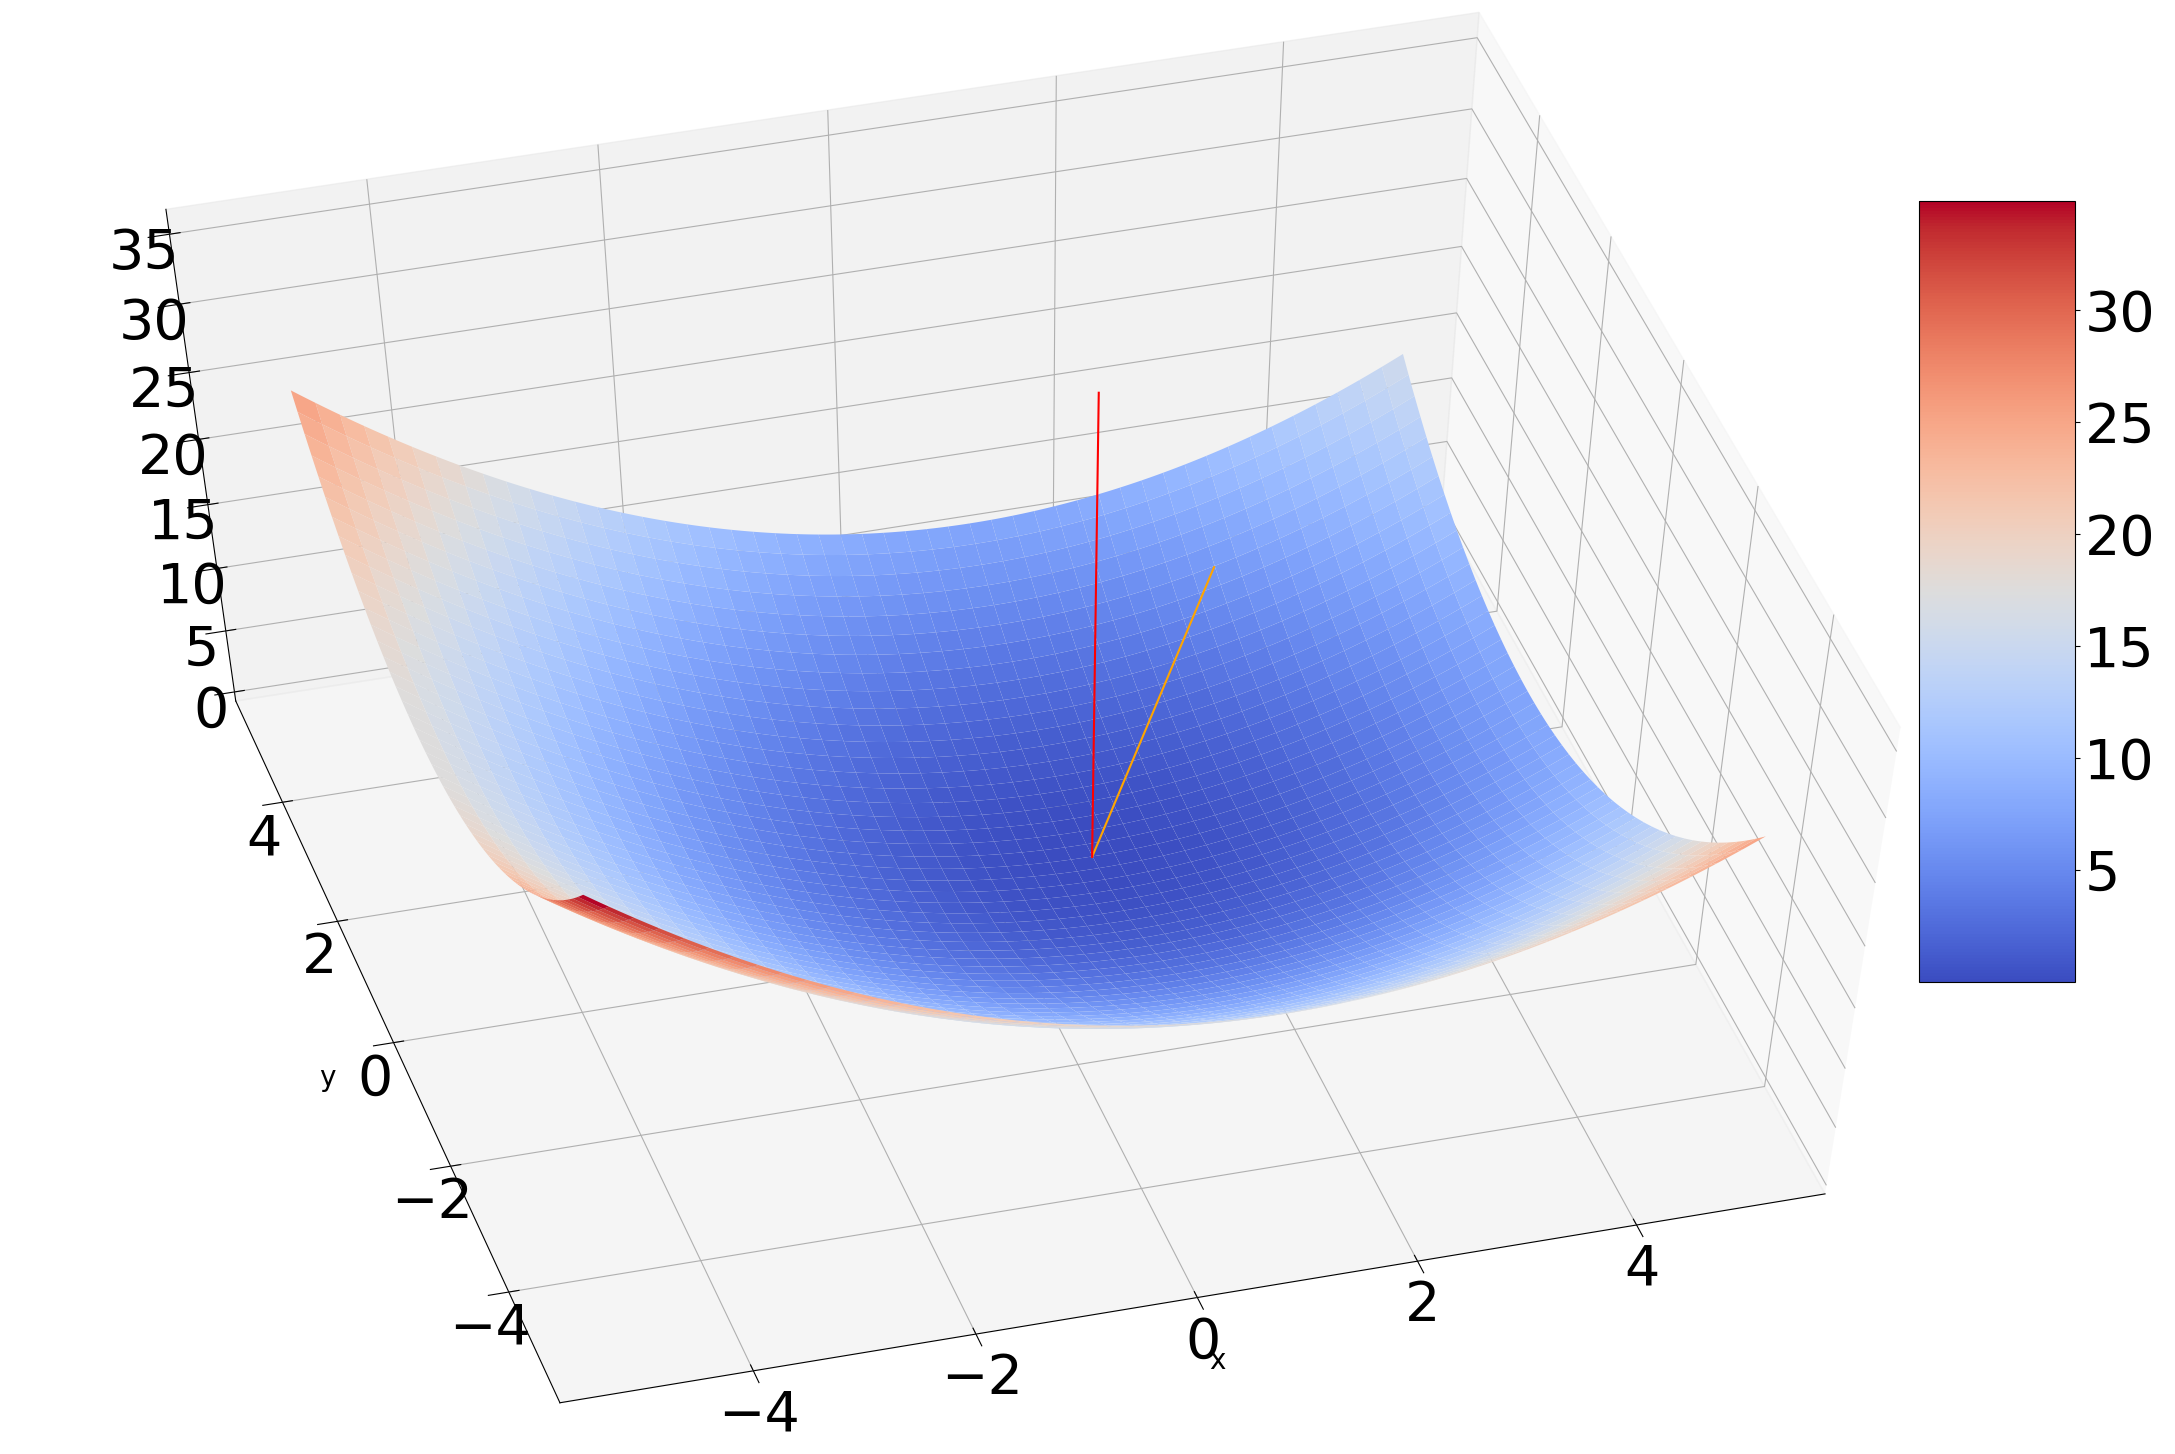
\includegraphics[width=0.7\textwidth]{Images/ConvOnce.png}
\caption{Gradient descent for $\lambda_1=\lambda_2=1$ and $\eta$ the optimal value of 1. It converges in one step.}
\label{Ideal}
\end{figure}

Now if the $\lambda_1 \neq \lambda_2$ we won't have a convergence. For both $r_{n,x}$ and $r_{n,y}$ will have a fixed value between 0 and 1, but not quite 0. So even after $10^5$ iterations we won't get the value to be exactly at the minimum, but ended up at x = 1.0000000000000002 and y = 1.0000000000000004 . In this case you could however say you're satisfied if you're within a certain range of the minimum. This we tested with $\lambda_1 = 10$, $\lambda_2 = 1$ and $\eta$ optimal.


\begin{figure}[H]
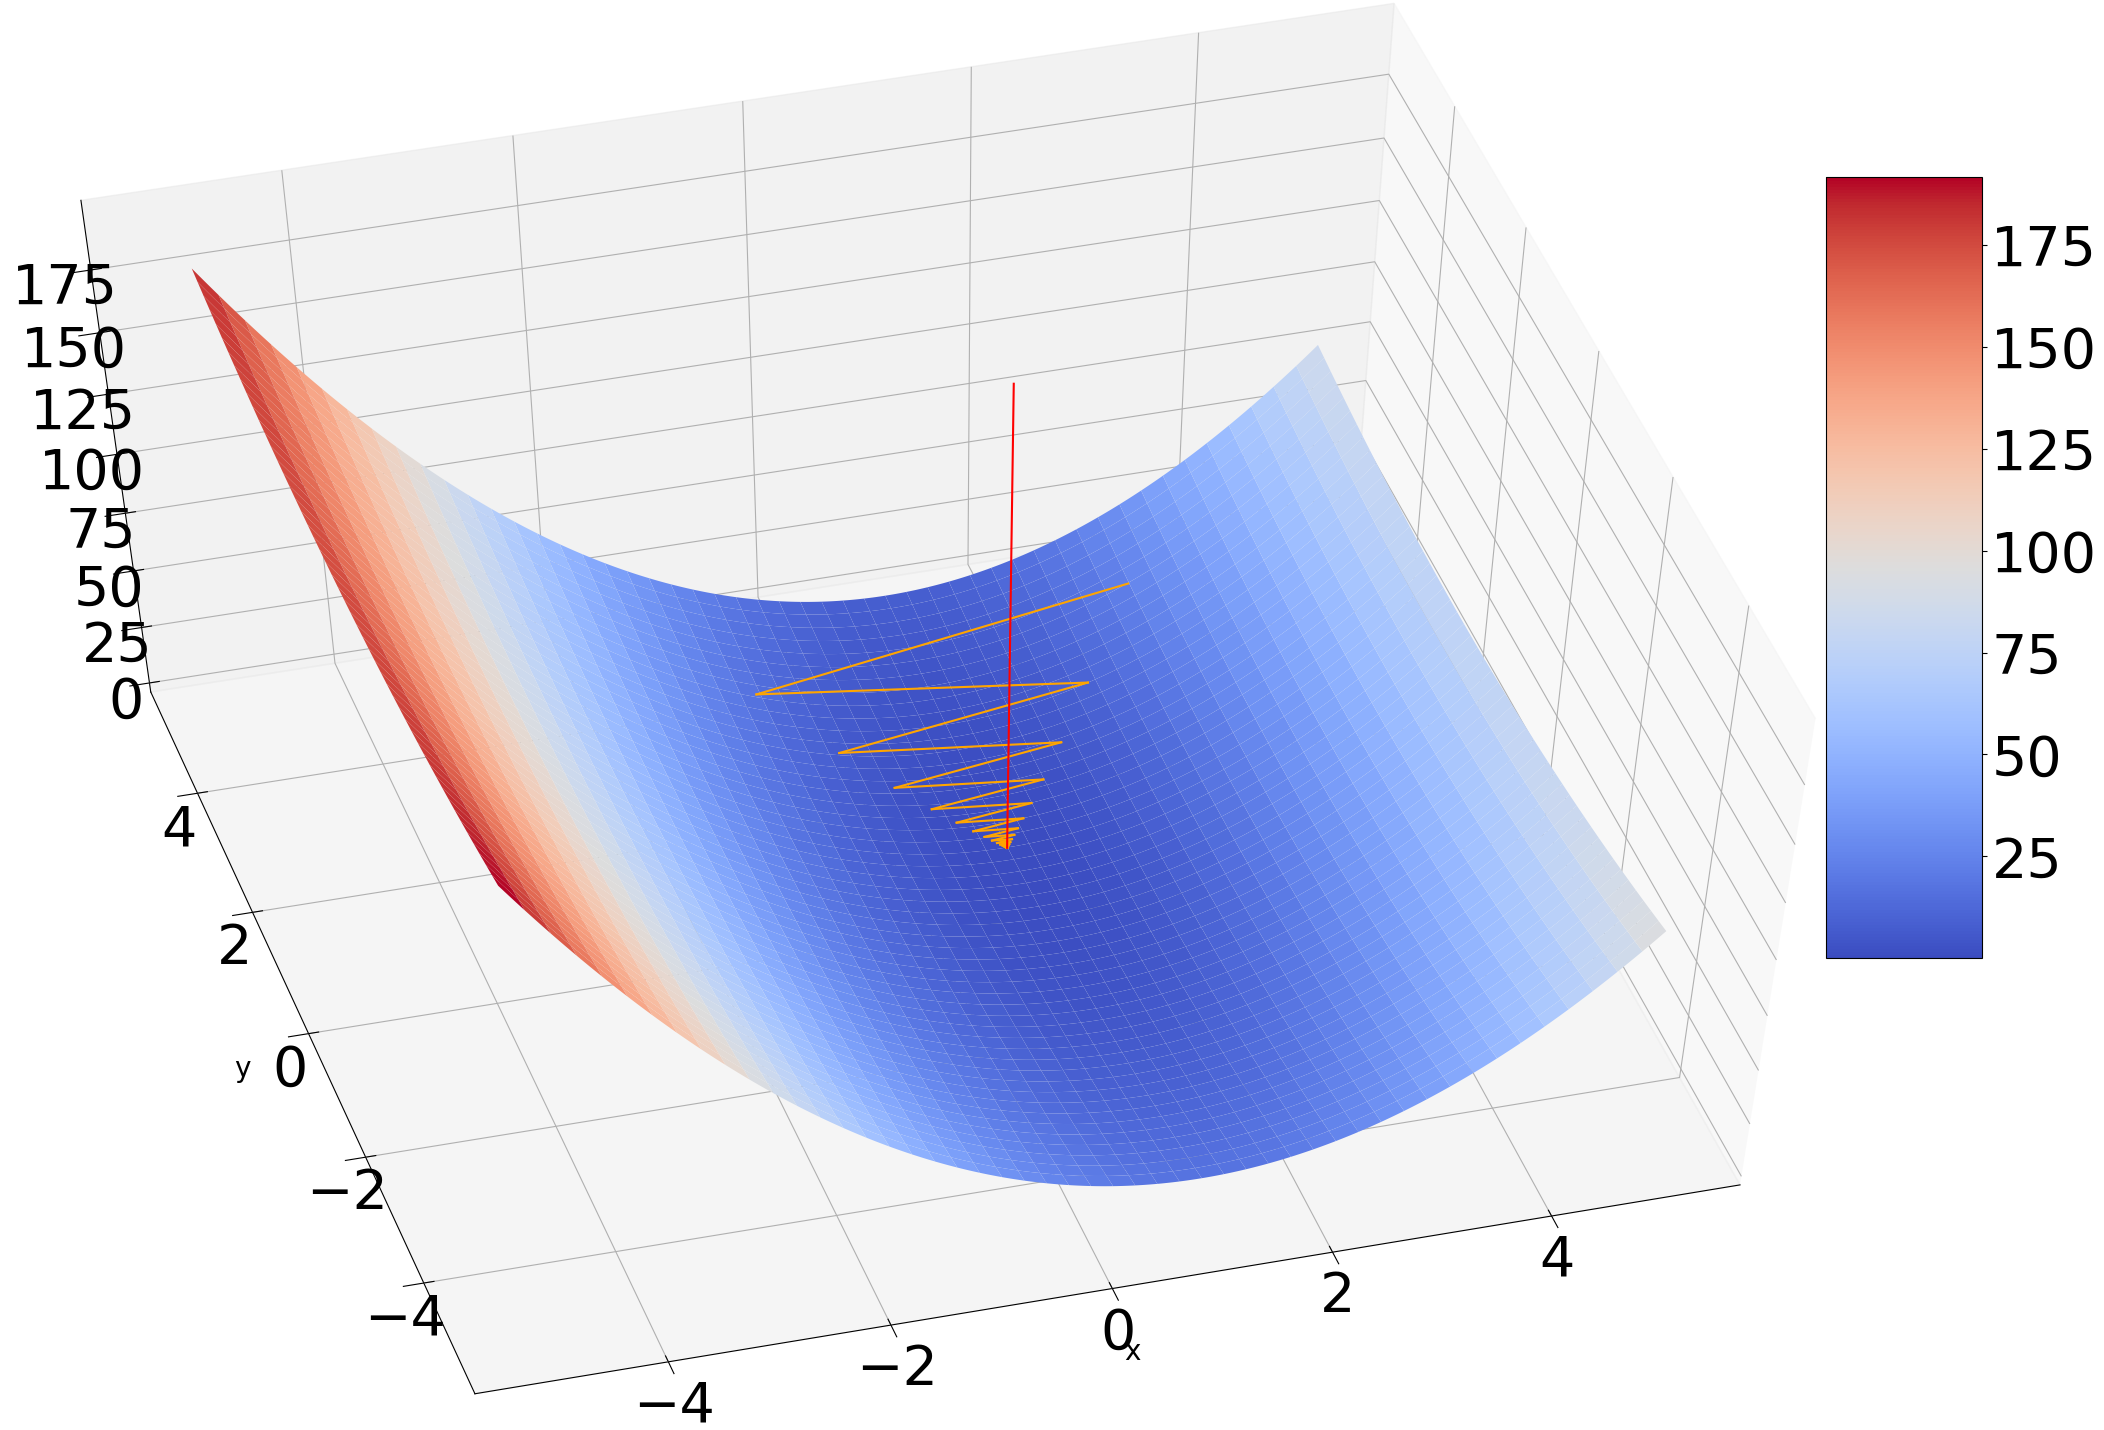
\includegraphics[width=0.7\textwidth]{Images/ConvMany.png}
\caption{Gradient descent for $\lambda_1 = 10$ and $\lambda_2 = 1$, with an optimal $\eta$. Notice how it overshoots for x, since $1-\eta\lambda_1 < 0$ . Vice versa it slowly converges in the y direction. This is because the if the subtraction $x_{n+1} - x^*$ flips sign, it will be on the other side of $x^*$. Therefore it will overshoot. And vice versa.}
\end{figure}

\newpage

We can also have the same situation as before, where it converges, but $\eta = \frac{\eta_{optimal}}{10} = \frac{1}{10} \frac{2}{\lambda_1+\lambda_2} = \frac{2}{110} = \frac{1}{55}$. Then we will have a slower converge. For example, in 100 steps it will still be at a distance of $r = \abs{x_n - x^*} + \abs{y_n - y^*} \approx 0.48$ while at the optimal rate it would be at distance $r \approx 9.6\cdot 10^{-9}$. This you can see at figure \ref{SlowConv}:


\begin{figure}[H]
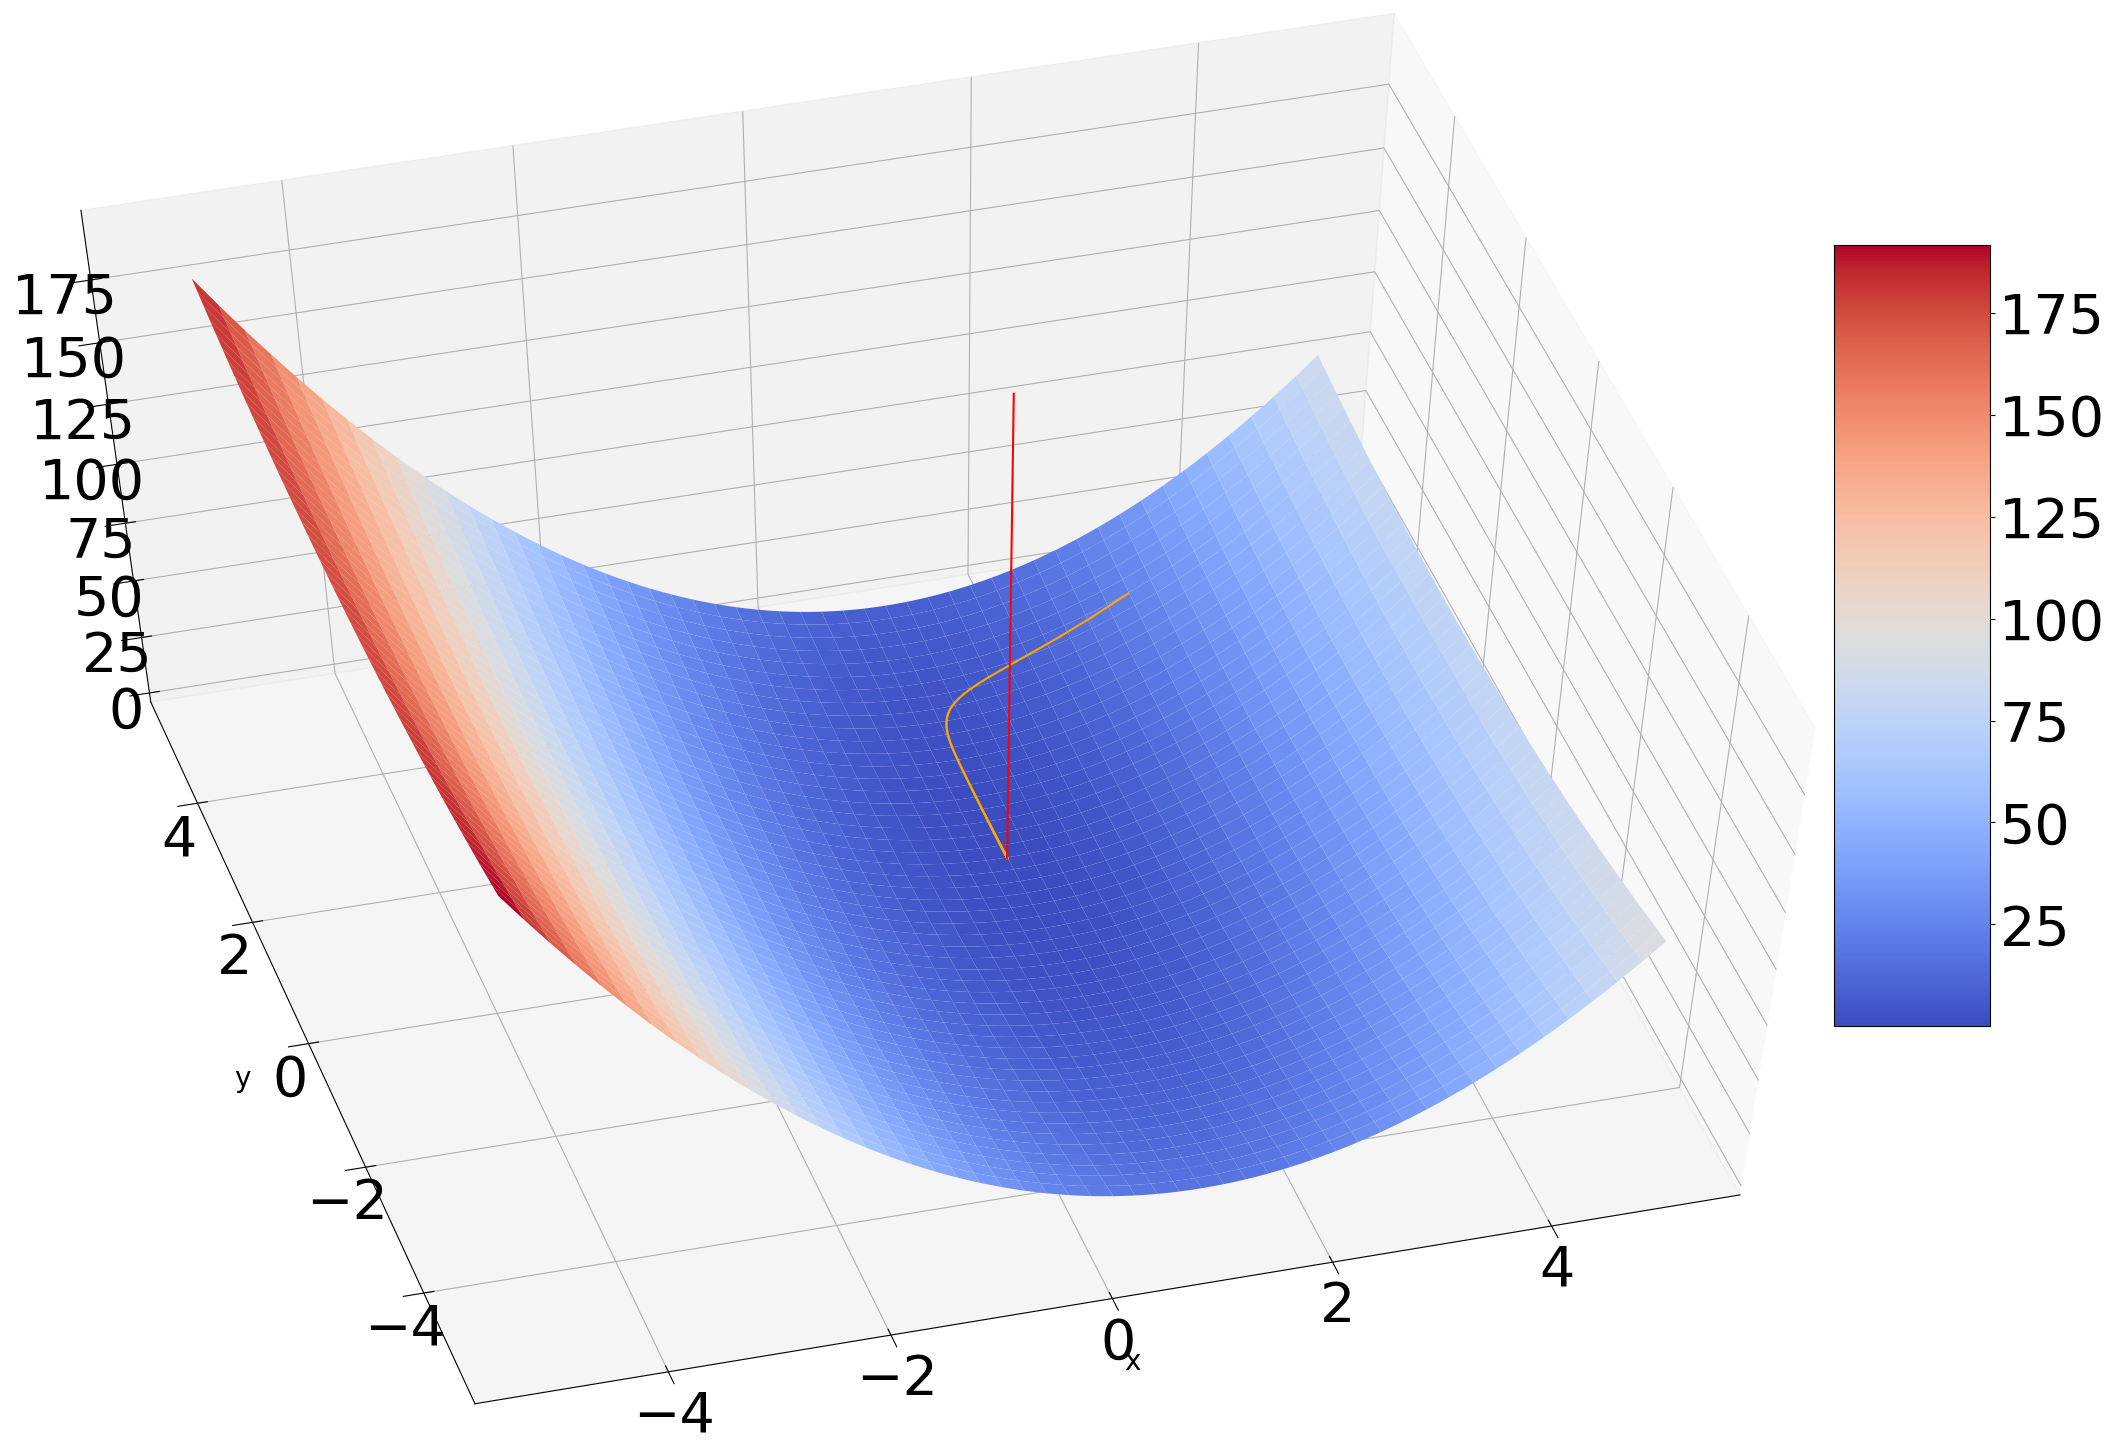
\includegraphics[width=0.7\textwidth]{Images/SlowConv}
\caption{Gradient descent which converges for the same parameters as at \ref{Ideal}, but with $\eta = \frac{\eta_{optimal}}{10}$. It looks smoother but it doesn't converge as fast.}
\label{SlowConv}
\end{figure} 
\newpage
What can also happen is that it converges in one dimension but diverges in another. This happens if $r_n=\abs{1-\eta \lambda}$ is smaller then 1 for one direction and greater then 1 for the other. For example, this happens for $\eta = 3$, $\lambda_1 = 1$ and $\lambda_2 = 0.5$. Then we will have $r_{n,x} = \abs{1-3} = 2$ and $r_{n,y} = \abs{1-1.5} = 0.5$. And since the sum in de absolute argument is negative for both, they will both jump over the minimum, but this is always the case for diverging paths since $\eta$ and $\lambda$ are both positive. This you can see in figure \ref{TopHalfConv}, where I have chosen the values for the $\lambda's$ I just mentioned, and the starting points are $x_0 = 3$ and $x_y =90$, so it is more evident it converges in y and diverges in x. Also, in this case $\eta$ should have been lower, it should have been $\eta_{optimal} = \frac{2}{\lambda_1+\lambda+2} = \frac{2}{1.5}< 2 < 3$. 

\begin{figure}[H]
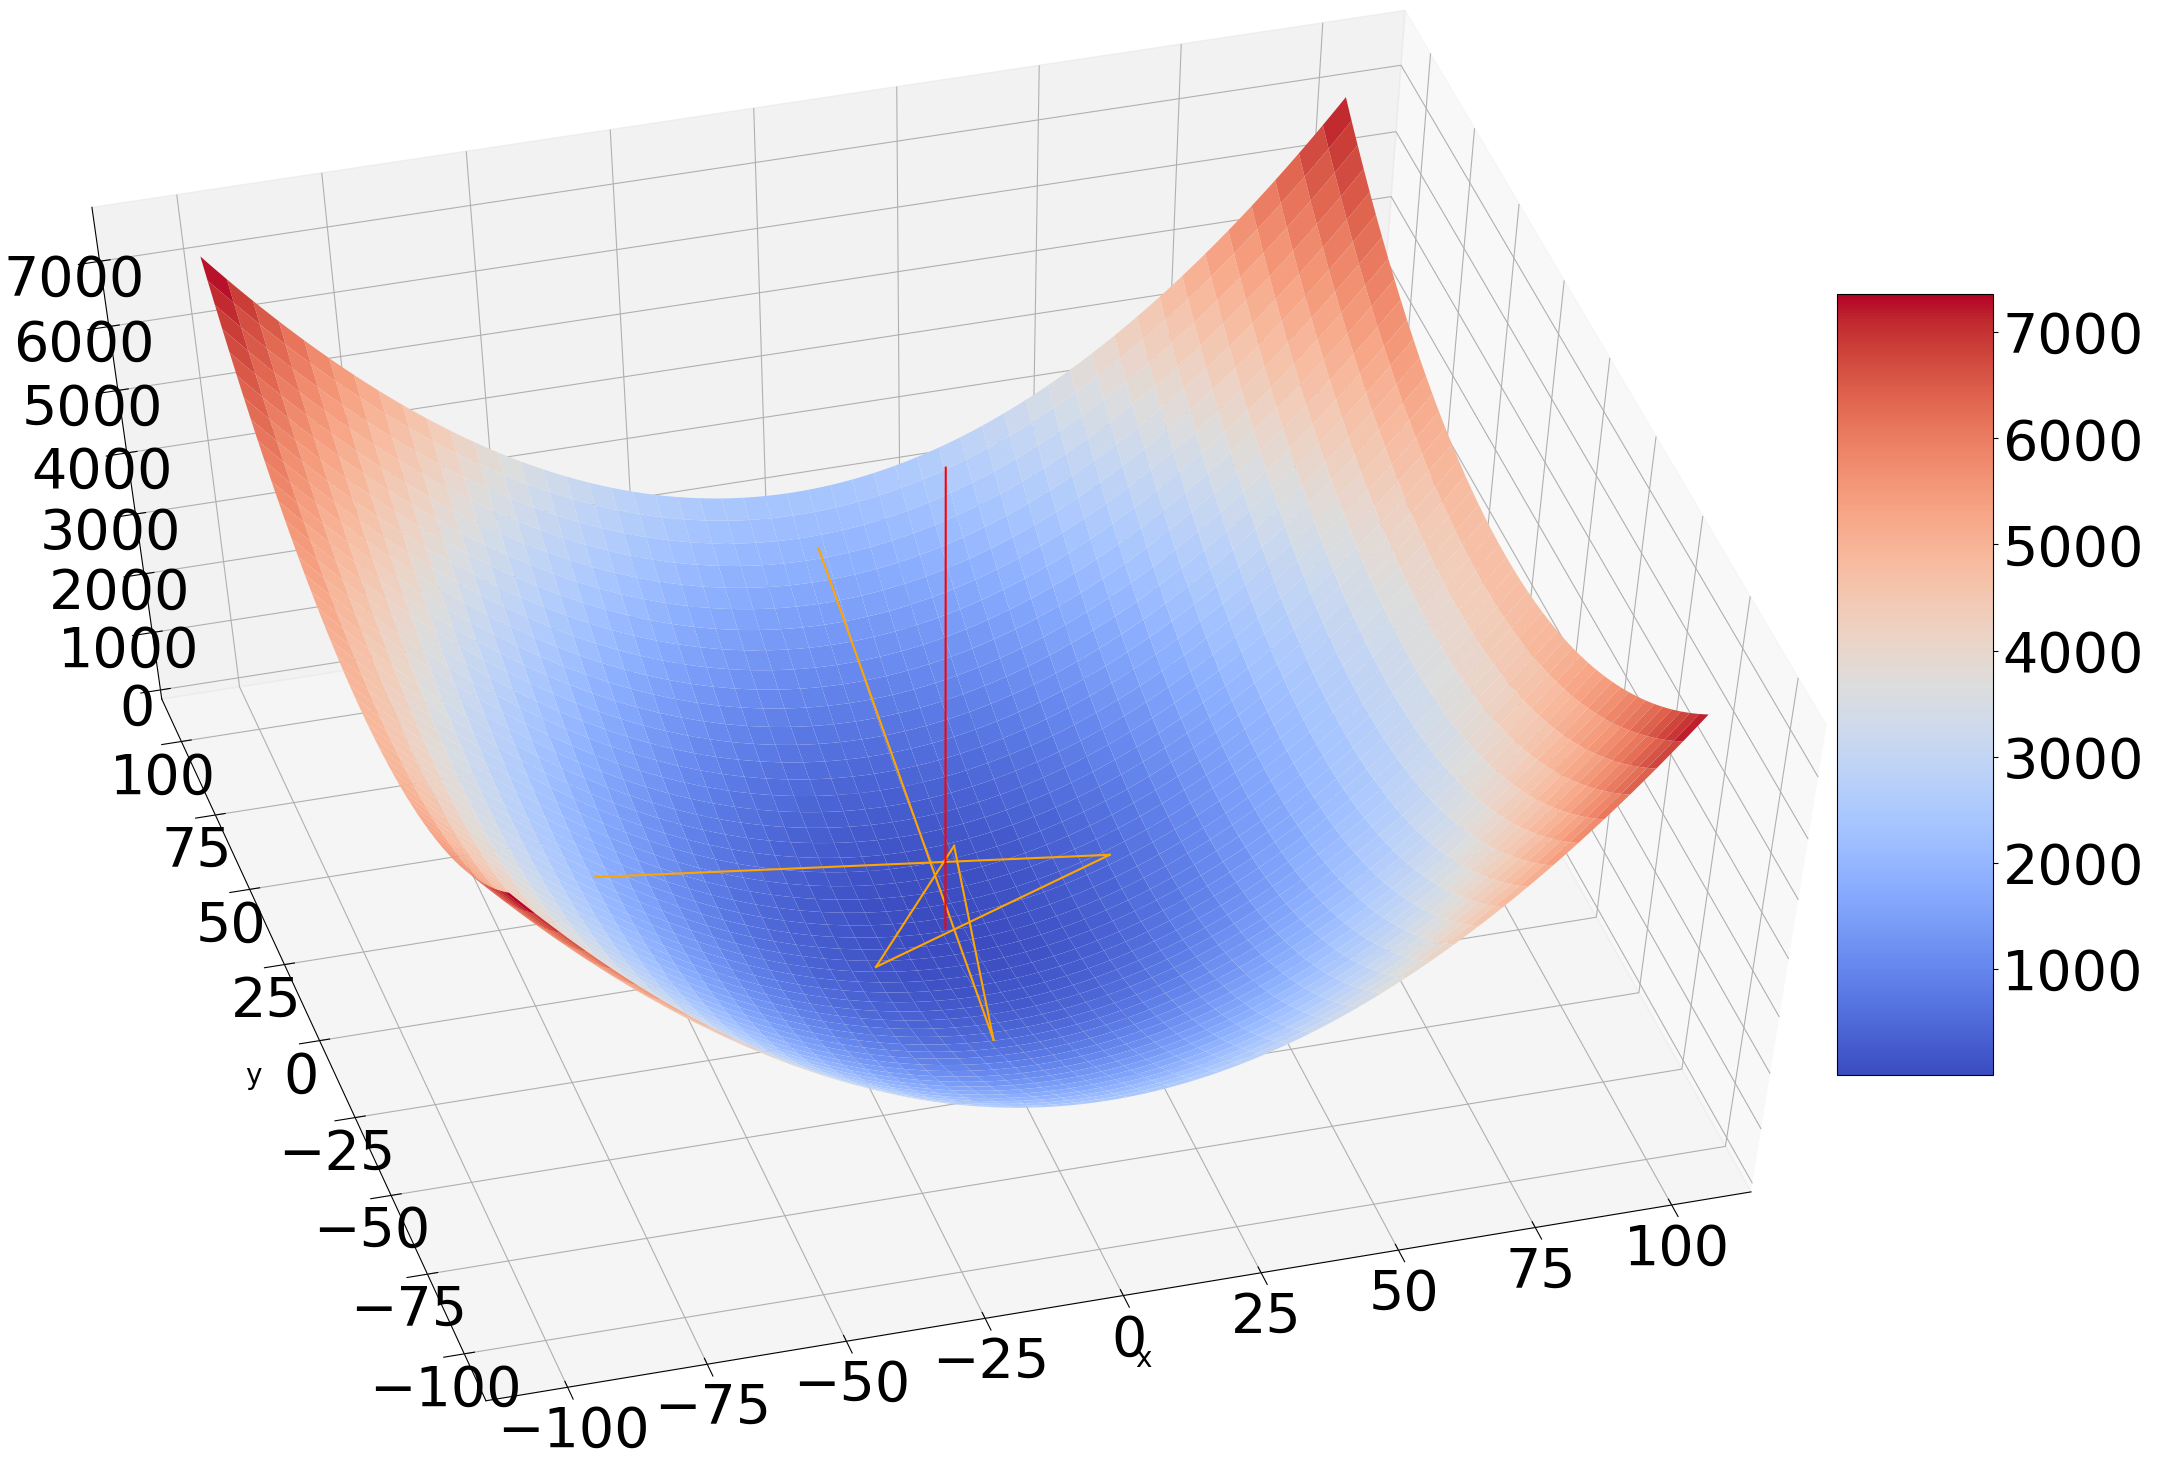
\includegraphics[width = 0.7\textwidth]{Images/TopHalfConv}
\caption{Gradient descent where it diverges in x and converges in y.}
\label{TopHalfConv}
\end{figure}

Now the final situation is when it diverges in both directions. If I fix $\eta = 1$ then it would happen for $\lambda_1 =3$, $ \lambda_2 = 2.5$. This you can see in figure \ref{BothDiverge}. 

\begin{figure}[H]
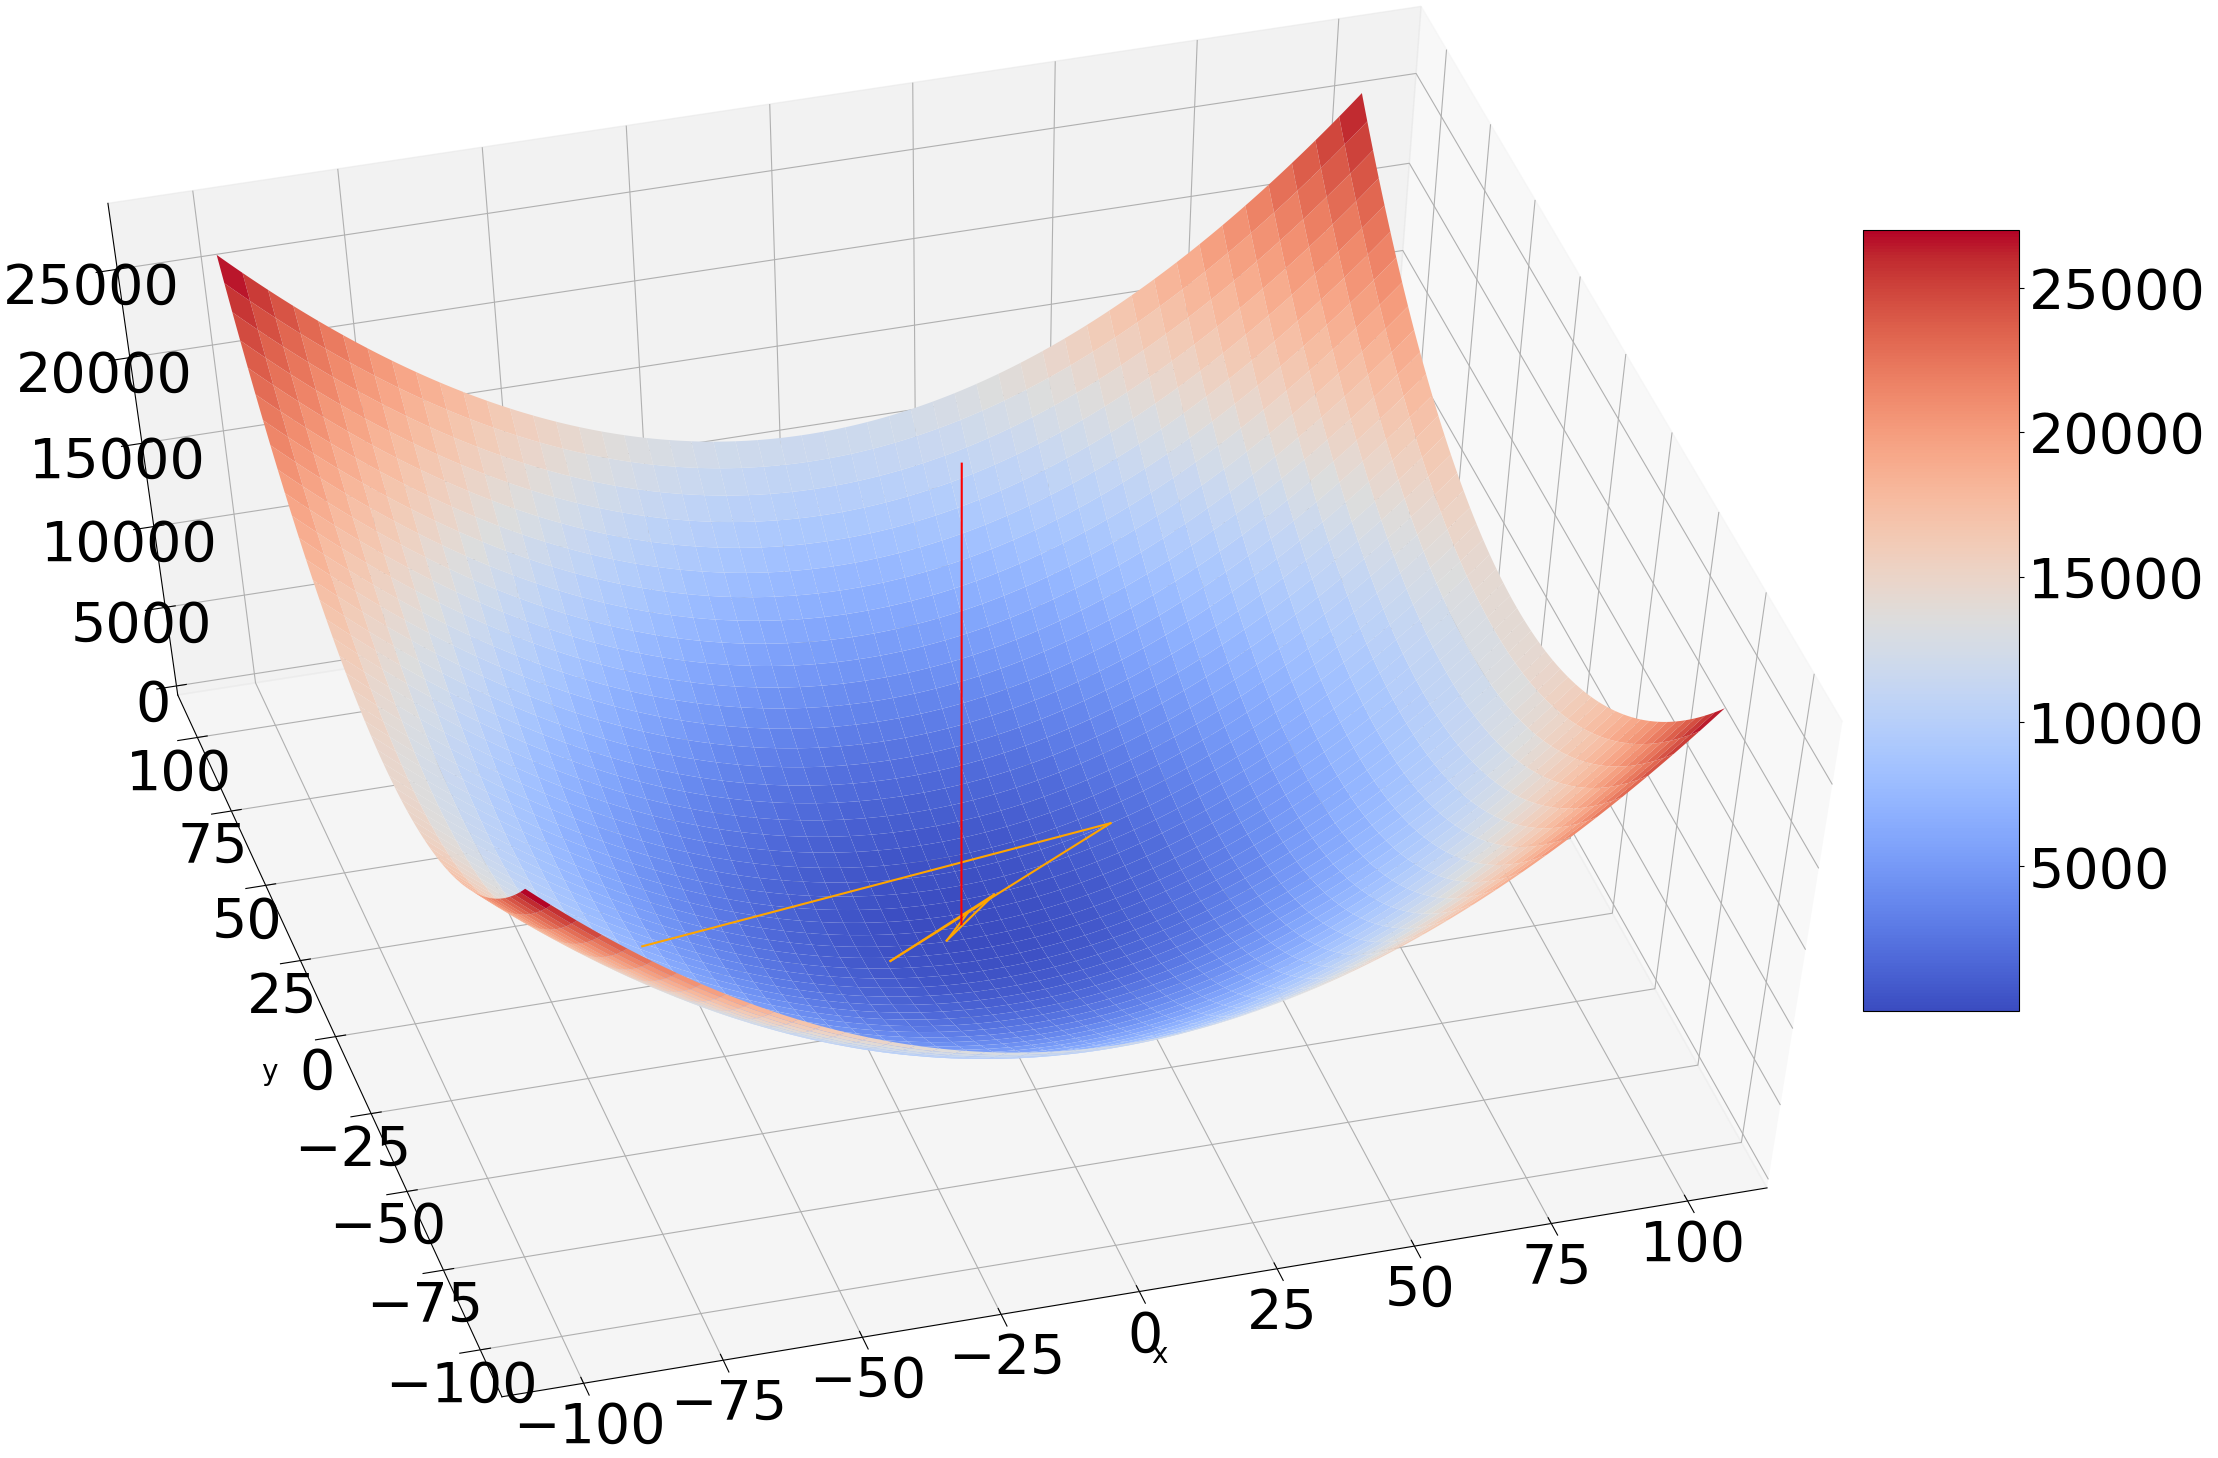
\includegraphics[width=0.7\textwidth]{Images/BothDiverge}
\caption{Gradient descent where it diverges in both x and y since $\lambda_1 = 3$, $\lambda_2 = 2.5$ and $\eta = 1$.}
\label{BothDiverge}
\end{figure} 



\end{document}
